%% FedLS-SQL manuscript: wrapper for the Journal of Intelligent Information
%% Systems (Springer Nature sn-jnl, version 3.1, December 2024).
%% The section bodies are in sections/ and use no command of this class.
%% `make submit` writes the single-file source the journal asks for.
\documentclass[pdflatex,sn-basic,Numbered]{sn-jnl}

%% Only the packages of the Springer template (the journal compiles on TeX Live 2018).
\usepackage{graphicx}
\usepackage{multirow}
\usepackage{amsmath,amssymb,amsfonts}
\usepackage{amsthm}
\usepackage{mathrsfs}
\usepackage[title]{appendix}
\usepackage{xcolor}
\usepackage{textcomp}
\usepackage{manyfoot}
\usepackage{booktabs}
\usepackage{algorithm}
\usepackage{algorithmicx}
\usepackage{algpseudocode}
\usepackage{listings}

%% Names and notation of the paper, written by hand. Result numbers and
%% settings are in generated/ and are never typed here.
\newcommand{\method}{FedLS-SQL}
% The writing tool named in the declaration on the use of AI tools.
\newcommand{\aitool}{Claude (Anthropic; model Claude Fable~5.2)}

%% Written by tools/paper_numbers.py from the committed evaluations. Do not edit.
\makeatletter
\newcommand{\pn@def}[2]{\expandafter\gdef\csname pn@\detokenize{#1}\endcsname{#2}}
\newcommand{\pn@get}[1]{\ifcsname pn@\detokenize{#1}\endcsname\csname pn@\detokenize{#1}\endcsname\else
  \textbf{??}\@latex@warning{No committed number for \detokenize{#1}}\fi}
%% a run: \ex[model]{set}{line}{round}; the model is the main model unless given
\newcommand{\ex}[4][qwen15]{\pn@get{ex/#1/#2/#3/#4}}
\newcommand{\lvl}[5][qwen15]{\pn@get{lvl/#1/#2/#3/#4/#5}}
\newcommand{\nerr}[4][qwen15]{\pn@get{err/#1/#2/#3/#4}}
\newcommand{\nwr}[4][qwen15]{\pn@get{wr/#1/#2/#3/#4}}
\newcommand{\ts}[4][qwen15]{\pn@get{ts/#1/#2/#3/#4}}
%% a comparison: \gain[model]{set}{line a}{round a}{line b}{round b}, b against a
\newcommand{\gain}[6][qwen15]{\pn@get{gain/#1/#2/#3/#4/#5/#6}}
\newcommand{\gap}[6][qwen15]{\pn@get{gap/#1/#2/#3/#4/#5/#6}}
\newcommand{\pval}[6][qwen15]{\pn@get{pval/#1/#2/#3/#4/#5/#6}}
\newcommand{\padj}[6][qwen15]{\pn@get{padj/#1/#2/#3/#4/#5/#6}}
\newcommand{\errpval}[6][qwen15]{\pn@get{errpval/#1/#2/#3/#4/#5/#6}}
\newcommand{\errpadj}[6][qwen15]{\pn@get{errpadj/#1/#2/#3/#4/#5/#6}}
\newcommand{\wrpval}[6][qwen15]{\pn@get{wrpval/#1/#2/#3/#4/#5/#6}}
\newcommand{\wrpadj}[6][qwen15]{\pn@get{wrpadj/#1/#2/#3/#4/#5/#6}}
\newcommand{\nfix}[6][qwen15]{\pn@get{nfix/#1/#2/#3/#4/#5/#6}}
\newcommand{\nbrk}[6][qwen15]{\pn@get{nbrk/#1/#2/#3/#4/#5/#6}}
\newcommand{\tsgain}[6][qwen15]{\pn@get{tsgain/#1/#2/#3/#4/#5/#6}}
\newcommand{\tsgap}[6][qwen15]{\pn@get{tsgap/#1/#2/#3/#4/#5/#6}}
\newcommand{\tspval}[6][qwen15]{\pn@get{tspval/#1/#2/#3/#4/#5/#6}}
\newcommand{\tspadj}[6][qwen15]{\pn@get{tspadj/#1/#2/#3/#4/#5/#6}}
%% a count or a cost: \fact{name}
\newcommand{\fact}[1]{\pn@get{fact/#1}}

\pn@def{ex/qwen15/bird/base/0}{29.47}
\pn@def{lvl/qwen15/bird/base/0/simple}{35.89}
\pn@def{lvl/qwen15/bird/base/0/moderate}{20.47}
\pn@def{lvl/qwen15/bird/base/0/challenging}{17.24}
\pn@def{err/qwen15/bird/base/0}{646}
\pn@def{wr/qwen15/bird/base/0}{436}
\pn@def{ts/qwen15/bird/base/0}{24.45}
\pn@def{ex/qwen15/bird/fedavg/1}{38.85}
\pn@def{lvl/qwen15/bird/fedavg/1/simple}{46.16}
\pn@def{lvl/qwen15/bird/fedavg/1/moderate}{28.66}
\pn@def{lvl/qwen15/bird/fedavg/1/challenging}{24.83}
\pn@def{err/qwen15/bird/fedavg/1}{372}
\pn@def{wr/qwen15/bird/fedavg/1}{566}
\pn@def{ts/qwen15/bird/fedavg/1}{32.99}
\pn@def{ex/qwen15/bird/fedavg/2}{42.70}
\pn@def{lvl/qwen15/bird/fedavg/2/simple}{50.49}
\pn@def{lvl/qwen15/bird/fedavg/2/moderate}{31.25}
\pn@def{lvl/qwen15/bird/fedavg/2/challenging}{29.66}
\pn@def{err/qwen15/bird/fedavg/2}{286}
\pn@def{wr/qwen15/bird/fedavg/2}{593}
\pn@def{ts/qwen15/bird/fedavg/2}{36.11}
\pn@def{ex/qwen15/bird/fedavg/3}{43.68}
\pn@def{lvl/qwen15/bird/fedavg/3/simple}{51.57}
\pn@def{lvl/qwen15/bird/fedavg/3/moderate}{32.54}
\pn@def{lvl/qwen15/bird/fedavg/3/challenging}{28.97}
\pn@def{err/qwen15/bird/fedavg/3}{276}
\pn@def{wr/qwen15/bird/fedavg/3}{588}
\pn@def{ts/qwen15/bird/fedavg/3}{37.22}
\pn@def{ex/qwen15/bird/fedavg/4}{42.57}
\pn@def{lvl/qwen15/bird/fedavg/4/simple}{51.35}
\pn@def{lvl/qwen15/bird/fedavg/4/moderate}{29.96}
\pn@def{lvl/qwen15/bird/fedavg/4/challenging}{26.90}
\pn@def{err/qwen15/bird/fedavg/4}{268}
\pn@def{wr/qwen15/bird/fedavg/4}{613}
\pn@def{ts/qwen15/bird/fedavg/4}{36.70}
\pn@def{ex/qwen15/bird/fedavgp/3}{43.16}
\pn@def{lvl/qwen15/bird/fedavgp/3/simple}{50.92}
\pn@def{lvl/qwen15/bird/fedavgp/3/moderate}{31.68}
\pn@def{lvl/qwen15/bird/fedavgp/3/challenging}{30.34}
\pn@def{err/qwen15/bird/fedavgp/3}{252}
\pn@def{wr/qwen15/bird/fedavgp/3}{620}
\pn@def{ts/qwen15/bird/fedavgp/3}{36.96}
\pn@def{ex/qwen15/bird/fedavgp/4}{43.09}
\pn@def{lvl/qwen15/bird/fedavgp/4/simple}{51.57}
\pn@def{lvl/qwen15/bird/fedavgp/4/moderate}{31.25}
\pn@def{lvl/qwen15/bird/fedavgp/4/challenging}{26.90}
\pn@def{err/qwen15/bird/fedavgp/4}{228}
\pn@def{wr/qwen15/bird/fedavgp/4}{645}
\pn@def{ts/qwen15/bird/fedavgp/4}{36.83}
\pn@def{ex/qwen15/bird/feddpo/3}{44.98}
\pn@def{lvl/qwen15/bird/feddpo/3/simple}{52.11}
\pn@def{lvl/qwen15/bird/feddpo/3/moderate}{35.34}
\pn@def{lvl/qwen15/bird/feddpo/3/challenging}{30.34}
\pn@def{err/qwen15/bird/feddpo/3}{133}
\pn@def{wr/qwen15/bird/feddpo/3}{711}
\pn@def{ts/qwen15/bird/feddpo/3}{38.92}
\pn@def{ex/qwen15/bird/feddpo/4}{45.50}
\pn@def{lvl/qwen15/bird/feddpo/4/simple}{52.54}
\pn@def{lvl/qwen15/bird/feddpo/4/moderate}{35.99}
\pn@def{lvl/qwen15/bird/feddpo/4/challenging}{31.03}
\pn@def{err/qwen15/bird/feddpo/4}{139}
\pn@def{wr/qwen15/bird/feddpo/4}{697}
\pn@def{ts/qwen15/bird/feddpo/4}{37.61}
\pn@def{ex/qwen15/bird/fixed/4}{46.15}
\pn@def{lvl/qwen15/bird/fixed/4/simple}{53.51}
\pn@def{lvl/qwen15/bird/fixed/4/moderate}{36.64}
\pn@def{lvl/qwen15/bird/fixed/4/challenging}{29.66}
\pn@def{err/qwen15/bird/fixed/4}{91}
\pn@def{wr/qwen15/bird/fixed/4}{735}
\pn@def{ts/qwen15/bird/fixed/4}{39.05}
\pn@def{ex/qwen15/bird/k2/3}{46.22}
\pn@def{lvl/qwen15/bird/k2/3/simple}{53.08}
\pn@def{lvl/qwen15/bird/k2/3/moderate}{36.85}
\pn@def{lvl/qwen15/bird/k2/3/challenging}{32.41}
\pn@def{err/qwen15/bird/k2/3}{102}
\pn@def{wr/qwen15/bird/k2/3}{723}
\pn@def{ts/qwen15/bird/k2/3}{39.05}
\pn@def{ex/qwen15/bird/k2/4}{48.76}
\pn@def{lvl/qwen15/bird/k2/4/simple}{56.00}
\pn@def{lvl/qwen15/bird/k2/4/moderate}{39.66}
\pn@def{lvl/qwen15/bird/k2/4/challenging}{31.72}
\pn@def{err/qwen15/bird/k2/4}{128}
\pn@def{wr/qwen15/bird/k2/4}{658}
\pn@def{ts/qwen15/bird/k2/4}{41.59}
\pn@def{ex/qwen15/bird/reagge/3}{46.02}
\pn@def{lvl/qwen15/bird/reagge/3/simple}{52.32}
\pn@def{lvl/qwen15/bird/reagge/3/moderate}{37.50}
\pn@def{lvl/qwen15/bird/reagge/3/challenging}{33.10}
\pn@def{err/qwen15/bird/reagge/3}{112}
\pn@def{wr/qwen15/bird/reagge/3}{716}
\pn@def{ts/qwen15/bird/reagge/3}{38.92}
\pn@def{ex/qwen15/bird/reaggq/3}{46.22}
\pn@def{lvl/qwen15/bird/reaggq/3/simple}{53.30}
\pn@def{lvl/qwen15/bird/reaggq/3/moderate}{37.07}
\pn@def{lvl/qwen15/bird/reaggq/3/challenging}{30.34}
\pn@def{err/qwen15/bird/reaggq/3}{105}
\pn@def{wr/qwen15/bird/reaggq/3}{720}
\pn@def{ts/qwen15/bird/reaggq/3}{39.31}
\pn@def{ex/qwen15/bird/rft/3}{44.39}
\pn@def{lvl/qwen15/bird/rft/3/simple}{51.78}
\pn@def{lvl/qwen15/bird/rft/3/moderate}{34.70}
\pn@def{lvl/qwen15/bird/rft/3/challenging}{28.28}
\pn@def{err/qwen15/bird/rft/3}{248}
\pn@def{wr/qwen15/bird/rft/3}{605}
\pn@def{ts/qwen15/bird/rft/3}{37.35}
\pn@def{ex/qwen15/bird/rft/4}{45.24}
\pn@def{lvl/qwen15/bird/rft/4/simple}{52.11}
\pn@def{lvl/qwen15/bird/rft/4/moderate}{36.64}
\pn@def{lvl/qwen15/bird/rft/4/challenging}{28.97}
\pn@def{err/qwen15/bird/rft/4}{228}
\pn@def{wr/qwen15/bird/rft/4}{612}
\pn@def{ts/qwen15/bird/rft/4}{38.20}
\pn@def{ex/qwen15/dk/base/0}{60.19}
\pn@def{lvl/qwen15/dk/base/0/easy}{80.00}
\pn@def{lvl/qwen15/dk/base/0/medium}{62.60}
\pn@def{lvl/qwen15/dk/base/0/hard}{47.30}
\pn@def{lvl/qwen15/dk/base/0/extra}{42.86}
\pn@def{err/qwen15/dk/base/0}{86}
\pn@def{wr/qwen15/dk/base/0}{127}
\pn@def{ex/qwen15/dk/fedavg/4}{59.63}
\pn@def{lvl/qwen15/dk/fedavg/4/easy}{72.73}
\pn@def{lvl/qwen15/dk/fedavg/4/medium}{63.01}
\pn@def{lvl/qwen15/dk/fedavg/4/hard}{44.59}
\pn@def{lvl/qwen15/dk/fedavg/4/extra}{48.57}
\pn@def{err/qwen15/dk/fedavg/4}{65}
\pn@def{wr/qwen15/dk/fedavg/4}{151}
\pn@def{ex/qwen15/dk/k0/4}{67.10}
\pn@def{lvl/qwen15/dk/k0/4/easy}{79.09}
\pn@def{lvl/qwen15/dk/k0/4/medium}{67.48}
\pn@def{lvl/qwen15/dk/k0/4/hard}{58.11}
\pn@def{lvl/qwen15/dk/k0/4/extra}{60.00}
\pn@def{err/qwen15/dk/k0/4}{33}
\pn@def{wr/qwen15/dk/k0/4}{143}
\pn@def{ex/qwen15/dk/k2/4}{63.55}
\pn@def{lvl/qwen15/dk/k2/4/easy}{78.18}
\pn@def{lvl/qwen15/dk/k2/4/medium}{64.63}
\pn@def{lvl/qwen15/dk/k2/4/hard}{48.65}
\pn@def{lvl/qwen15/dk/k2/4/extra}{56.19}
\pn@def{err/qwen15/dk/k2/4}{36}
\pn@def{wr/qwen15/dk/k2/4}{159}
\pn@def{ex/qwen15/realistic/base/0}{65.16}
\pn@def{lvl/qwen15/realistic/base/0/easy}{88.99}
\pn@def{lvl/qwen15/realistic/base/0/medium}{70.44}
\pn@def{lvl/qwen15/realistic/base/0/hard}{53.54}
\pn@def{lvl/qwen15/realistic/base/0/extra}{39.18}
\pn@def{err/qwen15/realistic/base/0}{72}
\pn@def{wr/qwen15/realistic/base/0}{105}
\pn@def{ts/qwen15/realistic/base/0}{51.18}
\pn@def{ex/qwen15/realistic/fedavg/4}{67.72}
\pn@def{lvl/qwen15/realistic/fedavg/4/easy}{88.07}
\pn@def{lvl/qwen15/realistic/fedavg/4/medium}{75.86}
\pn@def{lvl/qwen15/realistic/fedavg/4/hard}{53.54}
\pn@def{lvl/qwen15/realistic/fedavg/4/extra}{42.27}
\pn@def{err/qwen15/realistic/fedavg/4}{54}
\pn@def{wr/qwen15/realistic/fedavg/4}{110}
\pn@def{ts/qwen15/realistic/fedavg/4}{58.86}
\pn@def{ex/qwen15/realistic/k0/4}{71.26}
\pn@def{lvl/qwen15/realistic/k0/4/easy}{82.57}
\pn@def{lvl/qwen15/realistic/k0/4/medium}{77.83}
\pn@def{lvl/qwen15/realistic/k0/4/hard}{65.66}
\pn@def{lvl/qwen15/realistic/k0/4/extra}{50.52}
\pn@def{err/qwen15/realistic/k0/4}{32}
\pn@def{wr/qwen15/realistic/k0/4}{114}
\pn@def{ts/qwen15/realistic/k0/4}{57.09}
\pn@def{ex/qwen15/realistic/k2/4}{70.47}
\pn@def{lvl/qwen15/realistic/k2/4/easy}{84.40}
\pn@def{lvl/qwen15/realistic/k2/4/medium}{77.83}
\pn@def{lvl/qwen15/realistic/k2/4/hard}{61.62}
\pn@def{lvl/qwen15/realistic/k2/4/extra}{48.45}
\pn@def{err/qwen15/realistic/k2/4}{37}
\pn@def{wr/qwen15/realistic/k2/4}{113}
\pn@def{ts/qwen15/realistic/k2/4}{62.20}
\pn@def{ex/dsc13/spider/base/0}{55.85}
\pn@def{lvl/dsc13/spider/base/0/easy}{73.40}
\pn@def{lvl/dsc13/spider/base/0/medium}{61.84}
\pn@def{lvl/dsc13/spider/base/0/hard}{42.76}
\pn@def{lvl/dsc13/spider/base/0/extra}{35.29}
\pn@def{err/dsc13/spider/base/0}{152}
\pn@def{wr/dsc13/spider/base/0}{796}
\pn@def{ex/qwen05/spider/base/0}{54.40}
\pn@def{lvl/qwen05/spider/base/0/easy}{80.43}
\pn@def{lvl/qwen05/spider/base/0/medium}{60.09}
\pn@def{lvl/qwen05/spider/base/0/hard}{40.60}
\pn@def{lvl/qwen05/spider/base/0/extra}{24.37}
\pn@def{err/qwen05/spider/base/0}{470}
\pn@def{wr/qwen05/spider/base/0}{509}
\pn@def{ex/qwen05/spider/fedavg/4}{64.09}
\pn@def{lvl/qwen05/spider/fedavg/4/easy}{84.47}
\pn@def{lvl/qwen05/spider/fedavg/4/medium}{69.08}
\pn@def{lvl/qwen05/spider/fedavg/4/hard}{50.11}
\pn@def{lvl/qwen05/spider/fedavg/4/extra}{43.42}
\pn@def{err/qwen05/spider/fedavg/4}{365}
\pn@def{wr/qwen05/spider/fedavg/4}{406}
\pn@def{ex/qwen05/spider/k2/4}{66.19}
\pn@def{lvl/qwen05/spider/k2/4/easy}{84.04}
\pn@def{lvl/qwen05/spider/k2/4/medium}{70.95}
\pn@def{lvl/qwen05/spider/k2/4/hard}{55.08}
\pn@def{lvl/qwen05/spider/k2/4/extra}{45.66}
\pn@def{err/qwen05/spider/k2/4}{268}
\pn@def{wr/qwen05/spider/k2/4}{458}
\pn@def{ex/qwen15/spider/base/0}{68.05}
\pn@def{lvl/qwen15/spider/base/0/easy}{87.45}
\pn@def{lvl/qwen15/spider/base/0/medium}{71.41}
\pn@def{lvl/qwen15/spider/base/0/hard}{59.18}
\pn@def{lvl/qwen15/spider/base/0/extra}{45.94}
\pn@def{err/qwen15/spider/base/0}{287}
\pn@def{wr/qwen15/spider/base/0}{399}
\pn@def{ex/qwen15/spider/central/3}{75.03}
\pn@def{lvl/qwen15/spider/central/3/easy}{91.06}
\pn@def{lvl/qwen15/spider/central/3/medium}{78.30}
\pn@def{lvl/qwen15/spider/central/3/hard}{67.17}
\pn@def{lvl/qwen15/spider/central/3/extra}{56.30}
\pn@def{err/qwen15/spider/central/3}{159}
\pn@def{wr/qwen15/spider/central/3}{377}
\pn@def{ex/qwen15/spider/fedavg/1}{72.43}
\pn@def{lvl/qwen15/spider/fedavg/1/easy}{89.15}
\pn@def{lvl/qwen15/spider/fedavg/1/medium}{75.26}
\pn@def{lvl/qwen15/spider/fedavg/1/hard}{63.71}
\pn@def{lvl/qwen15/spider/fedavg/1/extra}{54.90}
\pn@def{err/qwen15/spider/fedavg/1}{215}
\pn@def{wr/qwen15/spider/fedavg/1}{377}
\pn@def{ex/qwen15/spider/fedavg/2}{74.10}
\pn@def{lvl/qwen15/spider/fedavg/2/easy}{89.36}
\pn@def{lvl/qwen15/spider/fedavg/2/medium}{78.65}
\pn@def{lvl/qwen15/spider/fedavg/2/hard}{65.23}
\pn@def{lvl/qwen15/spider/fedavg/2/extra}{54.62}
\pn@def{err/qwen15/spider/fedavg/2}{183}
\pn@def{wr/qwen15/spider/fedavg/2}{373}
\pn@def{ex/qwen15/spider/fedavg/3}{74.71}
\pn@def{lvl/qwen15/spider/fedavg/3/easy}{90.21}
\pn@def{lvl/qwen15/spider/fedavg/3/medium}{78.88}
\pn@def{lvl/qwen15/spider/fedavg/3/hard}{67.17}
\pn@def{lvl/qwen15/spider/fedavg/3/extra}{54.06}
\pn@def{err/qwen15/spider/fedavg/3}{164}
\pn@def{wr/qwen15/spider/fedavg/3}{379}
\pn@def{ex/qwen15/spider/fedavg/4}{74.71}
\pn@def{lvl/qwen15/spider/fedavg/4/easy}{90.64}
\pn@def{lvl/qwen15/spider/fedavg/4/medium}{78.18}
\pn@def{lvl/qwen15/spider/fedavg/4/hard}{66.74}
\pn@def{lvl/qwen15/spider/fedavg/4/extra}{55.74}
\pn@def{err/qwen15/spider/fedavg/4}{173}
\pn@def{wr/qwen15/spider/fedavg/4}{370}
\pn@def{ex/qwen15/spider/fedavg/5}{73.92}
\pn@def{lvl/qwen15/spider/fedavg/5/easy}{90.64}
\pn@def{lvl/qwen15/spider/fedavg/5/medium}{79.11}
\pn@def{lvl/qwen15/spider/fedavg/5/hard}{64.36}
\pn@def{lvl/qwen15/spider/fedavg/5/extra}{51.82}
\pn@def{err/qwen15/spider/fedavg/5}{188}
\pn@def{wr/qwen15/spider/fedavg/5}{372}
\pn@def{ex/qwen15/spider/fedavgp/3}{75.45}
\pn@def{lvl/qwen15/spider/fedavgp/3/easy}{90.43}
\pn@def{lvl/qwen15/spider/fedavgp/3/medium}{79.46}
\pn@def{lvl/qwen15/spider/fedavgp/3/hard}{68.03}
\pn@def{lvl/qwen15/spider/fedavgp/3/extra}{55.74}
\pn@def{err/qwen15/spider/fedavgp/3}{177}
\pn@def{wr/qwen15/spider/fedavgp/3}{350}
\pn@def{ex/qwen15/spider/fedavgp/4}{75.08}
\pn@def{lvl/qwen15/spider/fedavgp/4/easy}{90.43}
\pn@def{lvl/qwen15/spider/fedavgp/4/medium}{78.76}
\pn@def{lvl/qwen15/spider/fedavgp/4/hard}{66.52}
\pn@def{lvl/qwen15/spider/fedavgp/4/extra}{57.14}
\pn@def{err/qwen15/spider/fedavgp/4}{175}
\pn@def{wr/qwen15/spider/fedavgp/4}{360}
\pn@def{ex/qwen15/spider/feddpo/3}{73.59}
\pn@def{lvl/qwen15/spider/feddpo/3/easy}{88.94}
\pn@def{lvl/qwen15/spider/feddpo/3/medium}{75.50}
\pn@def{lvl/qwen15/spider/feddpo/3/hard}{68.03}
\pn@def{lvl/qwen15/spider/feddpo/3/extra}{56.02}
\pn@def{err/qwen15/spider/feddpo/3}{167}
\pn@def{wr/qwen15/spider/feddpo/3}{400}
\pn@def{ex/qwen15/spider/fixed/4}{78.02}
\pn@def{lvl/qwen15/spider/fixed/4/easy}{91.70}
\pn@def{lvl/qwen15/spider/fixed/4/medium}{81.56}
\pn@def{lvl/qwen15/spider/fixed/4/hard}{70.41}
\pn@def{lvl/qwen15/spider/fixed/4/extra}{61.34}
\pn@def{err/qwen15/spider/fixed/4}{97}
\pn@def{wr/qwen15/spider/fixed/4}{375}
\pn@def{ex/qwen15/spider/k0/4}{78.02}
\pn@def{lvl/qwen15/spider/k0/4/easy}{88.94}
\pn@def{lvl/qwen15/spider/k0/4/medium}{81.10}
\pn@def{lvl/qwen15/spider/k0/4/hard}{72.57}
\pn@def{lvl/qwen15/spider/k0/4/extra}{63.31}
\pn@def{err/qwen15/spider/k0/4}{69}
\pn@def{wr/qwen15/spider/k0/4}{403}
\pn@def{ex/qwen15/spider/k2/3}{77.46}
\pn@def{lvl/qwen15/spider/k2/3/easy}{91.49}
\pn@def{lvl/qwen15/spider/k2/3/medium}{80.63}
\pn@def{lvl/qwen15/spider/k2/3/hard}{71.06}
\pn@def{lvl/qwen15/spider/k2/3/extra}{59.66}
\pn@def{err/qwen15/spider/k2/3}{99}
\pn@def{wr/qwen15/spider/k2/3}{385}
\pn@def{ex/qwen15/spider/k2/4}{78.20}
\pn@def{lvl/qwen15/spider/k2/4/easy}{91.91}
\pn@def{lvl/qwen15/spider/k2/4/medium}{81.91}
\pn@def{lvl/qwen15/spider/k2/4/hard}{71.06}
\pn@def{lvl/qwen15/spider/k2/4/extra}{60.50}
\pn@def{err/qwen15/spider/k2/4}{84}
\pn@def{wr/qwen15/spider/k2/4}{384}
\pn@def{ex/qwen15/spider/k3/4}{77.97}
\pn@def{lvl/qwen15/spider/k3/4/easy}{91.28}
\pn@def{lvl/qwen15/spider/k3/4/medium}{80.86}
\pn@def{lvl/qwen15/spider/k3/4/hard}{72.35}
\pn@def{lvl/qwen15/spider/k3/4/extra}{60.78}
\pn@def{err/qwen15/spider/k3/4}{112}
\pn@def{wr/qwen15/spider/k3/4}{361}
\pn@def{ex/qwen15/spider/reagge/3}{76.94}
\pn@def{lvl/qwen15/spider/reagge/3/easy}{90.85}
\pn@def{lvl/qwen15/spider/reagge/3/medium}{80.40}
\pn@def{lvl/qwen15/spider/reagge/3/hard}{69.98}
\pn@def{lvl/qwen15/spider/reagge/3/extra}{59.38}
\pn@def{err/qwen15/spider/reagge/3}{106}
\pn@def{wr/qwen15/spider/reagge/3}{389}
\pn@def{ex/qwen15/spider/reaggq/3}{77.78}
\pn@def{lvl/qwen15/spider/reaggq/3/easy}{91.49}
\pn@def{lvl/qwen15/spider/reaggq/3/medium}{81.21}
\pn@def{lvl/qwen15/spider/reaggq/3/hard}{71.06}
\pn@def{lvl/qwen15/spider/reaggq/3/extra}{60.22}
\pn@def{err/qwen15/spider/reaggq/3}{99}
\pn@def{wr/qwen15/spider/reaggq/3}{378}
\pn@def{ex/qwen15/spider/rft/3}{75.87}
\pn@def{lvl/qwen15/spider/rft/3/easy}{90.43}
\pn@def{lvl/qwen15/spider/rft/3/medium}{79.35}
\pn@def{lvl/qwen15/spider/rft/3/hard}{67.60}
\pn@def{lvl/qwen15/spider/rft/3/extra}{59.10}
\pn@def{err/qwen15/spider/rft/3}{153}
\pn@def{wr/qwen15/spider/rft/3}{365}
\pn@def{ex/qwen15/spiderdev/base/0}{68.96}
\pn@def{lvl/qwen15/spiderdev/base/0/easy}{89.11}
\pn@def{lvl/qwen15/spiderdev/base/0/medium}{72.20}
\pn@def{lvl/qwen15/spiderdev/base/0/hard}{59.20}
\pn@def{lvl/qwen15/spiderdev/base/0/extra}{40.36}
\pn@def{err/qwen15/spiderdev/base/0}{154}
\pn@def{wr/qwen15/spiderdev/base/0}{167}
\pn@def{ts/qwen15/spiderdev/base/0}{58.32}
\pn@def{ex/qwen15/spiderdev/fedavg/4}{75.15}
\pn@def{lvl/qwen15/spiderdev/fedavg/4/easy}{88.71}
\pn@def{lvl/qwen15/spiderdev/fedavg/4/medium}{80.72}
\pn@def{lvl/qwen15/spiderdev/fedavg/4/hard}{63.22}
\pn@def{lvl/qwen15/spiderdev/fedavg/4/extra}{52.41}
\pn@def{err/qwen15/spiderdev/fedavg/4}{80}
\pn@def{wr/qwen15/spiderdev/fedavg/4}{177}
\pn@def{ts/qwen15/spiderdev/fedavg/4}{67.99}
\pn@def{ex/qwen15/spiderdev/k0/4}{77.27}
\pn@def{lvl/qwen15/spiderdev/k0/4/easy}{88.71}
\pn@def{lvl/qwen15/spiderdev/k0/4/medium}{79.37}
\pn@def{lvl/qwen15/spiderdev/k0/4/hard}{72.41}
\pn@def{lvl/qwen15/spiderdev/k0/4/extra}{59.64}
\pn@def{err/qwen15/spiderdev/k0/4}{50}
\pn@def{wr/qwen15/spiderdev/k0/4}{185}
\pn@def{ts/qwen15/spiderdev/k0/4}{67.21}
\pn@def{ex/qwen15/spiderdev/k2/4}{77.66}
\pn@def{lvl/qwen15/spiderdev/k2/4/easy}{90.32}
\pn@def{lvl/qwen15/spiderdev/k2/4/medium}{79.82}
\pn@def{lvl/qwen15/spiderdev/k2/4/hard}{68.39}
\pn@def{lvl/qwen15/spiderdev/k2/4/extra}{62.65}
\pn@def{err/qwen15/spiderdev/k2/4}{52}
\pn@def{wr/qwen15/spiderdev/k2/4}{179}
\pn@def{ts/qwen15/spiderdev/k2/4}{70.41}
\pn@def{ex/qwen15/syn/base/0}{56.77}
\pn@def{lvl/qwen15/syn/base/0/easy}{72.98}
\pn@def{lvl/qwen15/syn/base/0/medium}{59.32}
\pn@def{lvl/qwen15/syn/base/0/hard}{50.28}
\pn@def{lvl/qwen15/syn/base/0/extra}{33.14}
\pn@def{err/qwen15/syn/base/0}{218}
\pn@def{wr/qwen15/syn/base/0}{229}
\pn@def{ts/qwen15/syn/base/0}{46.23}
\pn@def{ex/qwen15/syn/fedavg/4}{59.09}
\pn@def{lvl/qwen15/syn/fedavg/4/easy}{72.18}
\pn@def{lvl/qwen15/syn/fedavg/4/medium}{60.68}
\pn@def{lvl/qwen15/syn/fedavg/4/hard}{55.37}
\pn@def{lvl/qwen15/syn/fedavg/4/extra}{39.64}
\pn@def{err/qwen15/syn/fedavg/4}{178}
\pn@def{wr/qwen15/syn/fedavg/4}{245}
\pn@def{ts/qwen15/syn/fedavg/4}{51.84}
\pn@def{ex/qwen15/syn/k0/4}{62.09}
\pn@def{lvl/qwen15/syn/k0/4/easy}{72.98}
\pn@def{lvl/qwen15/syn/k0/4/medium}{62.27}
\pn@def{lvl/qwen15/syn/k0/4/hard}{64.41}
\pn@def{lvl/qwen15/syn/k0/4/extra}{43.20}
\pn@def{err/qwen15/syn/k0/4}{103}
\pn@def{wr/qwen15/syn/k0/4}{289}
\pn@def{ts/qwen15/syn/k0/4}{51.35}
\pn@def{ex/qwen15/syn/k2/4}{62.96}
\pn@def{lvl/qwen15/syn/k2/4/easy}{74.19}
\pn@def{lvl/qwen15/syn/k2/4/medium}{62.95}
\pn@def{lvl/qwen15/syn/k2/4/hard}{61.02}
\pn@def{lvl/qwen15/syn/k2/4/extra}{48.52}
\pn@def{err/qwen15/syn/k2/4}{132}
\pn@def{wr/qwen15/syn/k2/4}{251}
\pn@def{ts/qwen15/syn/k2/4}{55.51}
\pn@def{gain/qwen15/bird/fedavg/1/k2/4}{+9.91}
\pn@def{gap/qwen15/bird/fedavg/1/k2/4}{9.91}
\pn@def{pval/qwen15/bird/fedavg/1/k2/4}{$8.4\times10^{-19}$}
\pn@def{padj/qwen15/bird/fedavg/1/k2/4}{$7.6\times10^{-18}$}
\pn@def{nfix/qwen15/bird/fedavg/1/k2/4}{228}
\pn@def{nbrk/qwen15/bird/fedavg/1/k2/4}{76}
\pn@def{tsgain/qwen15/bird/fedavg/1/k2/4}{+8.60}
\pn@def{tsgap/qwen15/bird/fedavg/1/k2/4}{8.60}
\pn@def{gain/qwen15/bird/fedavg/2/fedavg/3}{+0.98}
\pn@def{gap/qwen15/bird/fedavg/2/fedavg/3}{0.98}
\pn@def{nfix/qwen15/bird/fedavg/2/fedavg/3}{45}
\pn@def{nbrk/qwen15/bird/fedavg/2/fedavg/3}{30}
\pn@def{tsgain/qwen15/bird/fedavg/2/fedavg/3}{+1.11}
\pn@def{tsgap/qwen15/bird/fedavg/2/fedavg/3}{1.11}
\pn@def{gain/qwen15/bird/fedavg/2/feddpo/3}{+2.28}
\pn@def{gap/qwen15/bird/fedavg/2/feddpo/3}{2.28}
\pn@def{nfix/qwen15/bird/fedavg/2/feddpo/3}{165}
\pn@def{nbrk/qwen15/bird/fedavg/2/feddpo/3}{130}
\pn@def{tsgain/qwen15/bird/fedavg/2/feddpo/3}{+2.81}
\pn@def{tsgap/qwen15/bird/fedavg/2/feddpo/3}{2.81}
\pn@def{gain/qwen15/bird/fedavg/2/k2/3}{+3.52}
\pn@def{gap/qwen15/bird/fedavg/2/k2/3}{3.52}
\pn@def{nfix/qwen15/bird/fedavg/2/k2/3}{135}
\pn@def{nbrk/qwen15/bird/fedavg/2/k2/3}{81}
\pn@def{tsgain/qwen15/bird/fedavg/2/k2/3}{+2.94}
\pn@def{tsgap/qwen15/bird/fedavg/2/k2/3}{2.94}
\pn@def{gain/qwen15/bird/fedavg/2/k2/4}{+6.06}
\pn@def{gap/qwen15/bird/fedavg/2/k2/4}{6.06}
\pn@def{pval/qwen15/bird/fedavg/2/k2/4}{$3.4\times10^{-10}$}
\pn@def{padj/qwen15/bird/fedavg/2/k2/4}{$2.3\times10^{-9}$}
\pn@def{nfix/qwen15/bird/fedavg/2/k2/4}{157}
\pn@def{nbrk/qwen15/bird/fedavg/2/k2/4}{64}
\pn@def{tsgain/qwen15/bird/fedavg/2/k2/4}{+5.48}
\pn@def{tsgap/qwen15/bird/fedavg/2/k2/4}{5.48}
\pn@def{gain/qwen15/bird/fedavg/3/fedavgp/3}{$-$0.52}
\pn@def{gap/qwen15/bird/fedavg/3/fedavgp/3}{0.52}
\pn@def{nfix/qwen15/bird/fedavg/3/fedavgp/3}{38}
\pn@def{nbrk/qwen15/bird/fedavg/3/fedavgp/3}{46}
\pn@def{tsgain/qwen15/bird/fedavg/3/fedavgp/3}{$-$0.26}
\pn@def{tsgap/qwen15/bird/fedavg/3/fedavgp/3}{0.26}
\pn@def{gain/qwen15/bird/fedavg/3/k2/3}{+2.54}
\pn@def{gap/qwen15/bird/fedavg/3/k2/3}{2.54}
\pn@def{pval/qwen15/bird/fedavg/3/k2/3}{0.0087}
\pn@def{padj/qwen15/bird/fedavg/3/k2/3}{0.044}
\pn@def{nfix/qwen15/bird/fedavg/3/k2/3}{125}
\pn@def{nbrk/qwen15/bird/fedavg/3/k2/3}{86}
\pn@def{tsgain/qwen15/bird/fedavg/3/k2/3}{+1.83}
\pn@def{tsgap/qwen15/bird/fedavg/3/k2/3}{1.83}
\pn@def{tspval/qwen15/bird/fedavg/3/k2/3}{0.0499}
\pn@def{tspadj/qwen15/bird/fedavg/3/k2/3}{0.15}
\pn@def{gain/qwen15/bird/fedavg/3/k2/4}{+5.08}
\pn@def{gap/qwen15/bird/fedavg/3/k2/4}{5.08}
\pn@def{pval/qwen15/bird/fedavg/3/k2/4}{$4.9\times10^{-8}$}
\pn@def{padj/qwen15/bird/fedavg/3/k2/4}{$1.9\times10^{-7}$}
\pn@def{nfix/qwen15/bird/fedavg/3/k2/4}{141}
\pn@def{nbrk/qwen15/bird/fedavg/3/k2/4}{63}
\pn@def{tsgain/qwen15/bird/fedavg/3/k2/4}{+4.37}
\pn@def{tsgap/qwen15/bird/fedavg/3/k2/4}{4.37}
\pn@def{gain/qwen15/bird/fedavg/4/base/0}{$-$13.10}
\pn@def{gap/qwen15/bird/fedavg/4/base/0}{13.10}
\pn@def{pval/qwen15/bird/fedavg/4/base/0}{$1.2\times10^{-27}$}
\pn@def{padj/qwen15/bird/fedavg/4/base/0}{$8.4\times10^{-27}$}
\pn@def{nfix/qwen15/bird/fedavg/4/base/0}{78}
\pn@def{nbrk/qwen15/bird/fedavg/4/base/0}{279}
\pn@def{tsgain/qwen15/bird/fedavg/4/base/0}{$-$12.25}
\pn@def{tsgap/qwen15/bird/fedavg/4/base/0}{12.25}
\pn@def{gain/qwen15/bird/fedavg/4/fedavgp/4}{+0.52}
\pn@def{gap/qwen15/bird/fedavg/4/fedavgp/4}{0.52}
\pn@def{nfix/qwen15/bird/fedavg/4/fedavgp/4}{57}
\pn@def{nbrk/qwen15/bird/fedavg/4/fedavgp/4}{49}
\pn@def{tsgain/qwen15/bird/fedavg/4/fedavgp/4}{+0.13}
\pn@def{tsgap/qwen15/bird/fedavg/4/fedavgp/4}{0.13}
\pn@def{gain/qwen15/bird/fedavg/4/feddpo/4}{+2.93}
\pn@def{gap/qwen15/bird/fedavg/4/feddpo/4}{2.93}
\pn@def{pval/qwen15/bird/fedavg/4/feddpo/4}{0.0072}
\pn@def{padj/qwen15/bird/fedavg/4/feddpo/4}{0.014}
\pn@def{nfix/qwen15/bird/fedavg/4/feddpo/4}{157}
\pn@def{nbrk/qwen15/bird/fedavg/4/feddpo/4}{112}
\pn@def{tsgain/qwen15/bird/fedavg/4/feddpo/4}{+0.91}
\pn@def{tsgap/qwen15/bird/fedavg/4/feddpo/4}{0.91}
\pn@def{gain/qwen15/bird/fedavg/4/k2/4}{+6.19}
\pn@def{gap/qwen15/bird/fedavg/4/k2/4}{6.19}
\pn@def{pval/qwen15/bird/fedavg/4/k2/4}{$4.6\times10^{-11}$}
\pn@def{padj/qwen15/bird/fedavg/4/k2/4}{$2.3\times10^{-10}$}
\pn@def{nfix/qwen15/bird/fedavg/4/k2/4}{153}
\pn@def{nbrk/qwen15/bird/fedavg/4/k2/4}{58}
\pn@def{tsgain/qwen15/bird/fedavg/4/k2/4}{+4.89}
\pn@def{tsgap/qwen15/bird/fedavg/4/k2/4}{4.89}
\pn@def{tspval/qwen15/bird/fedavg/4/k2/4}{$4.2\times10^{-8}$}
\pn@def{tspadj/qwen15/bird/fedavg/4/k2/4}{$3.7\times10^{-7}$}
\pn@def{gain/qwen15/bird/fedavg/4/rft/4}{+2.67}
\pn@def{gap/qwen15/bird/fedavg/4/rft/4}{2.67}
\pn@def{nfix/qwen15/bird/fedavg/4/rft/4}{94}
\pn@def{nbrk/qwen15/bird/fedavg/4/rft/4}{53}
\pn@def{tsgain/qwen15/bird/fedavg/4/rft/4}{+1.50}
\pn@def{tsgap/qwen15/bird/fedavg/4/rft/4}{1.50}
\pn@def{gain/qwen15/bird/feddpo/3/feddpo/4}{+0.52}
\pn@def{gap/qwen15/bird/feddpo/3/feddpo/4}{0.52}
\pn@def{nfix/qwen15/bird/feddpo/3/feddpo/4}{64}
\pn@def{nbrk/qwen15/bird/feddpo/3/feddpo/4}{56}
\pn@def{tsgain/qwen15/bird/feddpo/3/feddpo/4}{$-$1.31}
\pn@def{tsgap/qwen15/bird/feddpo/3/feddpo/4}{1.31}
\pn@def{gain/qwen15/bird/feddpo/4/fixed/4}{+0.65}
\pn@def{gap/qwen15/bird/feddpo/4/fixed/4}{0.65}
\pn@def{nfix/qwen15/bird/feddpo/4/fixed/4}{83}
\pn@def{nbrk/qwen15/bird/feddpo/4/fixed/4}{73}
\pn@def{tsgain/qwen15/bird/feddpo/4/fixed/4}{+1.44}
\pn@def{tsgap/qwen15/bird/feddpo/4/fixed/4}{1.44}
\pn@def{gain/qwen15/bird/k2/3/fedavgp/3}{$-$3.06}
\pn@def{gap/qwen15/bird/k2/3/fedavgp/3}{3.06}
\pn@def{pval/qwen15/bird/k2/3/fedavgp/3}{0.0014}
\pn@def{padj/qwen15/bird/k2/3/fedavgp/3}{0.0098}
\pn@def{nfix/qwen15/bird/k2/3/fedavgp/3}{81}
\pn@def{nbrk/qwen15/bird/k2/3/fedavgp/3}{128}
\pn@def{tsgain/qwen15/bird/k2/3/fedavgp/3}{$-$2.09}
\pn@def{tsgap/qwen15/bird/k2/3/fedavgp/3}{2.09}
\pn@def{tspval/qwen15/bird/k2/3/fedavgp/3}{0.023}
\pn@def{tspadj/qwen15/bird/k2/3/fedavgp/3}{0.091}
\pn@def{gain/qwen15/bird/k2/3/feddpo/3}{$-$1.24}
\pn@def{gap/qwen15/bird/k2/3/feddpo/3}{1.24}
\pn@def{pval/qwen15/bird/k2/3/feddpo/3}{0.17}
\pn@def{padj/qwen15/bird/k2/3/feddpo/3}{0.33}
\pn@def{nfix/qwen15/bird/k2/3/feddpo/3}{75}
\pn@def{nbrk/qwen15/bird/k2/3/feddpo/3}{94}
\pn@def{tsgain/qwen15/bird/k2/3/feddpo/3}{$-$0.13}
\pn@def{tsgap/qwen15/bird/k2/3/feddpo/3}{0.13}
\pn@def{tspval/qwen15/bird/k2/3/feddpo/3}{0.94}
\pn@def{tspadj/qwen15/bird/k2/3/feddpo/3}{0.94}
\pn@def{gain/qwen15/bird/k2/3/k2/4}{+2.54}
\pn@def{gap/qwen15/bird/k2/3/k2/4}{2.54}
\pn@def{pval/qwen15/bird/k2/3/k2/4}{$2.1\times10^{-4}$}
\pn@def{padj/qwen15/bird/k2/3/k2/4}{$4.1\times10^{-4}$}
\pn@def{nfix/qwen15/bird/k2/3/k2/4}{73}
\pn@def{nbrk/qwen15/bird/k2/3/k2/4}{34}
\pn@def{tsgain/qwen15/bird/k2/3/k2/4}{+2.54}
\pn@def{tsgap/qwen15/bird/k2/3/k2/4}{2.54}
\pn@def{gain/qwen15/bird/k2/3/rft/3}{$-$1.83}
\pn@def{gap/qwen15/bird/k2/3/rft/3}{1.83}
\pn@def{pval/qwen15/bird/k2/3/rft/3}{0.057}
\pn@def{padj/qwen15/bird/k2/3/rft/3}{0.17}
\pn@def{nfix/qwen15/bird/k2/3/rft/3}{87}
\pn@def{nbrk/qwen15/bird/k2/3/rft/3}{115}
\pn@def{tsgain/qwen15/bird/k2/3/rft/3}{$-$1.70}
\pn@def{tsgap/qwen15/bird/k2/3/rft/3}{1.70}
\pn@def{tspval/qwen15/bird/k2/3/rft/3}{0.062}
\pn@def{tspadj/qwen15/bird/k2/3/rft/3}{0.15}
\pn@def{gain/qwen15/bird/k2/4/fedavgp/4}{$-$5.67}
\pn@def{gap/qwen15/bird/k2/4/fedavgp/4}{5.67}
\pn@def{pval/qwen15/bird/k2/4/fedavgp/4}{$1.9\times10^{-9}$}
\pn@def{padj/qwen15/bird/k2/4/fedavgp/4}{$2.7\times10^{-8}$}
\pn@def{nfix/qwen15/bird/k2/4/fedavgp/4}{62}
\pn@def{nbrk/qwen15/bird/k2/4/fedavgp/4}{149}
\pn@def{tsgain/qwen15/bird/k2/4/fedavgp/4}{$-$4.76}
\pn@def{tsgap/qwen15/bird/k2/4/fedavgp/4}{4.76}
\pn@def{tspval/qwen15/bird/k2/4/fedavgp/4}{$2.5\times10^{-7}$}
\pn@def{tspadj/qwen15/bird/k2/4/fedavgp/4}{$2.0\times10^{-6}$}
\pn@def{gain/qwen15/bird/k2/4/feddpo/4}{$-$3.26}
\pn@def{gap/qwen15/bird/k2/4/feddpo/4}{3.26}
\pn@def{pval/qwen15/bird/k2/4/feddpo/4}{$1.4\times10^{-4}$}
\pn@def{padj/qwen15/bird/k2/4/feddpo/4}{0.0013}
\pn@def{nfix/qwen15/bird/k2/4/feddpo/4}{59}
\pn@def{nbrk/qwen15/bird/k2/4/feddpo/4}{109}
\pn@def{tsgain/qwen15/bird/k2/4/feddpo/4}{$-$3.98}
\pn@def{tsgap/qwen15/bird/k2/4/feddpo/4}{3.98}
\pn@def{tspval/qwen15/bird/k2/4/feddpo/4}{$6.8\times10^{-6}$}
\pn@def{tspadj/qwen15/bird/k2/4/feddpo/4}{$4.8\times10^{-5}$}
\pn@def{gain/qwen15/bird/k2/4/fixed/4}{$-$2.61}
\pn@def{gap/qwen15/bird/k2/4/fixed/4}{2.61}
\pn@def{pval/qwen15/bird/k2/4/fixed/4}{$5.7\times10^{-4}$}
\pn@def{padj/qwen15/bird/k2/4/fixed/4}{0.0046}
\pn@def{nfix/qwen15/bird/k2/4/fixed/4}{45}
\pn@def{nbrk/qwen15/bird/k2/4/fixed/4}{85}
\pn@def{tsgain/qwen15/bird/k2/4/fixed/4}{$-$2.54}
\pn@def{tsgap/qwen15/bird/k2/4/fixed/4}{2.54}
\pn@def{tspval/qwen15/bird/k2/4/fixed/4}{$6.2\times10^{-4}$}
\pn@def{tspadj/qwen15/bird/k2/4/fixed/4}{0.0031}
\pn@def{gain/qwen15/bird/k2/4/rft/4}{$-$3.52}
\pn@def{gap/qwen15/bird/k2/4/rft/4}{3.52}
\pn@def{pval/qwen15/bird/k2/4/rft/4}{$5.2\times10^{-5}$}
\pn@def{padj/qwen15/bird/k2/4/rft/4}{$5.7\times10^{-4}$}
\pn@def{nfix/qwen15/bird/k2/4/rft/4}{60}
\pn@def{nbrk/qwen15/bird/k2/4/rft/4}{114}
\pn@def{tsgain/qwen15/bird/k2/4/rft/4}{$-$3.39}
\pn@def{tsgap/qwen15/bird/k2/4/rft/4}{3.39}
\pn@def{tspval/qwen15/bird/k2/4/rft/4}{$9.0\times10^{-5}$}
\pn@def{tspadj/qwen15/bird/k2/4/rft/4}{$5.4\times10^{-4}$}
\pn@def{gain/qwen15/dk/fedavg/4/k2/4}{+3.92}
\pn@def{gap/qwen15/dk/fedavg/4/k2/4}{3.92}
\pn@def{pval/qwen15/dk/fedavg/4/k2/4}{0.017}
\pn@def{padj/qwen15/dk/fedavg/4/k2/4}{0.15}
\pn@def{nfix/qwen15/dk/fedavg/4/k2/4}{46}
\pn@def{nbrk/qwen15/dk/fedavg/4/k2/4}{25}
\pn@def{gain/qwen15/dk/k0/4/k2/4}{$-$3.55}
\pn@def{gap/qwen15/dk/k0/4/k2/4}{3.55}
\pn@def{pval/qwen15/dk/k0/4/k2/4}{0.032}
\pn@def{padj/qwen15/dk/k0/4/k2/4}{0.19}
\pn@def{nfix/qwen15/dk/k0/4/k2/4}{26}
\pn@def{nbrk/qwen15/dk/k0/4/k2/4}{45}
\pn@def{gain/qwen15/realistic/fedavg/4/k2/4}{+2.75}
\pn@def{gap/qwen15/realistic/fedavg/4/k2/4}{2.75}
\pn@def{pval/qwen15/realistic/fedavg/4/k2/4}{0.10}
\pn@def{padj/qwen15/realistic/fedavg/4/k2/4}{0.41}
\pn@def{nfix/qwen15/realistic/fedavg/4/k2/4}{39}
\pn@def{nbrk/qwen15/realistic/fedavg/4/k2/4}{25}
\pn@def{tsgain/qwen15/realistic/fedavg/4/k2/4}{+3.34}
\pn@def{tsgap/qwen15/realistic/fedavg/4/k2/4}{3.34}
\pn@def{tspval/qwen15/realistic/fedavg/4/k2/4}{0.036}
\pn@def{tspadj/qwen15/realistic/fedavg/4/k2/4}{0.19}
\pn@def{gain/qwen15/realistic/k0/4/k2/4}{$-$0.79}
\pn@def{gap/qwen15/realistic/k0/4/k2/4}{0.79}
\pn@def{pval/qwen15/realistic/k0/4/k2/4}{0.72}
\pn@def{padj/qwen15/realistic/k0/4/k2/4}{1.00}
\pn@def{nfix/qwen15/realistic/k0/4/k2/4}{32}
\pn@def{nbrk/qwen15/realistic/k0/4/k2/4}{36}
\pn@def{tsgain/qwen15/realistic/k0/4/k2/4}{+5.11}
\pn@def{tsgap/qwen15/realistic/k0/4/k2/4}{5.11}
\pn@def{tspval/qwen15/realistic/k0/4/k2/4}{0.0067}
\pn@def{tspadj/qwen15/realistic/k0/4/k2/4}{0.073}
\pn@def{gain/qwen05/spider/fedavg/4/k2/4}{+2.10}
\pn@def{gap/qwen05/spider/fedavg/4/k2/4}{2.10}
\pn@def{pval/qwen05/spider/fedavg/4/k2/4}{0.0056}
\pn@def{padj/qwen05/spider/fedavg/4/k2/4}{0.0056}
\pn@def{nfix/qwen05/spider/fedavg/4/k2/4}{149}
\pn@def{nbrk/qwen05/spider/fedavg/4/k2/4}{104}
\pn@def{gain/qwen15/spider/central/3/k2/4}{+3.17}
\pn@def{gap/qwen15/spider/central/3/k2/4}{3.17}
\pn@def{pval/qwen15/spider/central/3/k2/4}{$2.4\times10^{-5}$}
\pn@def{padj/qwen15/spider/central/3/k2/4}{$7.1\times10^{-5}$}
\pn@def{nfix/qwen15/spider/central/3/k2/4}{161}
\pn@def{nbrk/qwen15/spider/central/3/k2/4}{93}
\pn@def{gain/qwen15/spider/fedavg/1/k2/4}{+5.77}
\pn@def{gap/qwen15/spider/fedavg/1/k2/4}{5.77}
\pn@def{pval/qwen15/spider/fedavg/1/k2/4}{$1.9\times10^{-14}$}
\pn@def{padj/qwen15/spider/fedavg/1/k2/4}{$1.6\times10^{-13}$}
\pn@def{nfix/qwen15/spider/fedavg/1/k2/4}{196}
\pn@def{nbrk/qwen15/spider/fedavg/1/k2/4}{72}
\pn@def{gain/qwen15/spider/fedavg/2/fedavg/3}{+0.61}
\pn@def{gap/qwen15/spider/fedavg/2/fedavg/3}{0.61}
\pn@def{nfix/qwen15/spider/fedavg/2/fedavg/3}{61}
\pn@def{nbrk/qwen15/spider/fedavg/2/fedavg/3}{48}
\pn@def{gain/qwen15/spider/fedavg/2/k2/3}{+3.36}
\pn@def{gap/qwen15/spider/fedavg/2/k2/3}{3.36}
\pn@def{nfix/qwen15/spider/fedavg/2/k2/3}{146}
\pn@def{nbrk/qwen15/spider/fedavg/2/k2/3}{74}
\pn@def{gain/qwen15/spider/fedavg/2/k2/4}{+4.10}
\pn@def{gap/qwen15/spider/fedavg/2/k2/4}{4.10}
\pn@def{pval/qwen15/spider/fedavg/2/k2/4}{$1.9\times10^{-9}$}
\pn@def{padj/qwen15/spider/fedavg/2/k2/4}{$1.2\times10^{-8}$}
\pn@def{nfix/qwen15/spider/fedavg/2/k2/4}{152}
\pn@def{nbrk/qwen15/spider/fedavg/2/k2/4}{64}
\pn@def{gain/qwen15/spider/fedavg/3/fedavgp/3}{+0.74}
\pn@def{gap/qwen15/spider/fedavg/3/fedavgp/3}{0.74}
\pn@def{nfix/qwen15/spider/fedavg/3/fedavgp/3}{51}
\pn@def{nbrk/qwen15/spider/fedavg/3/fedavgp/3}{35}
\pn@def{gain/qwen15/spider/fedavg/3/k2/3}{+2.75}
\pn@def{gap/qwen15/spider/fedavg/3/k2/3}{2.75}
\pn@def{pval/qwen15/spider/fedavg/3/k2/3}{$5.4\times10^{-5}$}
\pn@def{padj/qwen15/spider/fedavg/3/k2/3}{$5.7\times10^{-4}$}
\pn@def{nfix/qwen15/spider/fedavg/3/k2/3}{134}
\pn@def{nbrk/qwen15/spider/fedavg/3/k2/3}{75}
\pn@def{gain/qwen15/spider/fedavg/3/k2/4}{+3.49}
\pn@def{gap/qwen15/spider/fedavg/3/k2/4}{3.49}
\pn@def{pval/qwen15/spider/fedavg/3/k2/4}{$2.3\times10^{-7}$}
\pn@def{padj/qwen15/spider/fedavg/3/k2/4}{$6.9\times10^{-7}$}
\pn@def{nfix/qwen15/spider/fedavg/3/k2/4}{142}
\pn@def{nbrk/qwen15/spider/fedavg/3/k2/4}{67}
\pn@def{gain/qwen15/spider/fedavg/4/base/0}{$-$6.66}
\pn@def{gap/qwen15/spider/fedavg/4/base/0}{6.66}
\pn@def{pval/qwen15/spider/fedavg/4/base/0}{$1.4\times10^{-15}$}
\pn@def{padj/qwen15/spider/fedavg/4/base/0}{$8.6\times10^{-15}$}
\pn@def{nfix/qwen15/spider/fedavg/4/base/0}{92}
\pn@def{nbrk/qwen15/spider/fedavg/4/base/0}{235}
\pn@def{gain/qwen15/spider/fedavg/4/central/3}{+0.32}
\pn@def{gap/qwen15/spider/fedavg/4/central/3}{0.32}
\pn@def{pval/qwen15/spider/fedavg/4/central/3}{0.69}
\pn@def{padj/qwen15/spider/fedavg/4/central/3}{0.69}
\pn@def{nfix/qwen15/spider/fedavg/4/central/3}{113}
\pn@def{nbrk/qwen15/spider/fedavg/4/central/3}{106}
\pn@def{gain/qwen15/spider/fedavg/4/fedavgp/4}{+0.37}
\pn@def{gap/qwen15/spider/fedavg/4/fedavgp/4}{0.37}
\pn@def{nfix/qwen15/spider/fedavg/4/fedavgp/4}{66}
\pn@def{nbrk/qwen15/spider/fedavg/4/fedavgp/4}{58}
\pn@def{gain/qwen15/spider/fedavg/4/k0/4}{+3.31}
\pn@def{gap/qwen15/spider/fedavg/4/k0/4}{3.31}
\pn@def{nfix/qwen15/spider/fedavg/4/k0/4}{178}
\pn@def{nbrk/qwen15/spider/fedavg/4/k0/4}{107}
\pn@def{gain/qwen15/spider/fedavg/4/k2/4}{+3.49}
\pn@def{gap/qwen15/spider/fedavg/4/k2/4}{3.49}
\pn@def{pval/qwen15/spider/fedavg/4/k2/4}{$6.4\times10^{-7}$}
\pn@def{padj/qwen15/spider/fedavg/4/k2/4}{$2.6\times10^{-6}$}
\pn@def{nfix/qwen15/spider/fedavg/4/k2/4}{150}
\pn@def{nbrk/qwen15/spider/fedavg/4/k2/4}{75}
\pn@def{gain/qwen15/spider/fedavg/4/k3/4}{+3.26}
\pn@def{gap/qwen15/spider/fedavg/4/k3/4}{3.26}
\pn@def{nfix/qwen15/spider/fedavg/4/k3/4}{146}
\pn@def{nbrk/qwen15/spider/fedavg/4/k3/4}{76}
\pn@def{gain/qwen15/spider/fedavg/5/k2/4}{+4.28}
\pn@def{gap/qwen15/spider/fedavg/5/k2/4}{4.28}
\pn@def{pval/qwen15/spider/fedavg/5/k2/4}{$2.3\times10^{-9}$}
\pn@def{padj/qwen15/spider/fedavg/5/k2/4}{$1.2\times10^{-8}$}
\pn@def{nfix/qwen15/spider/fedavg/5/k2/4}{165}
\pn@def{nbrk/qwen15/spider/fedavg/5/k2/4}{73}
\pn@def{gain/qwen15/spider/k2/3/fedavgp/3}{$-$2.01}
\pn@def{gap/qwen15/spider/k2/3/fedavgp/3}{2.01}
\pn@def{pval/qwen15/spider/k2/3/fedavgp/3}{0.0036}
\pn@def{padj/qwen15/spider/k2/3/fedavgp/3}{0.021}
\pn@def{nfix/qwen15/spider/k2/3/fedavgp/3}{83}
\pn@def{nbrk/qwen15/spider/k2/3/fedavgp/3}{126}
\pn@def{gain/qwen15/spider/k2/3/feddpo/3}{$-$3.87}
\pn@def{gap/qwen15/spider/k2/3/feddpo/3}{3.87}
\pn@def{pval/qwen15/spider/k2/3/feddpo/3}{$7.6\times10^{-9}$}
\pn@def{padj/qwen15/spider/k2/3/feddpo/3}{$9.9\times10^{-8}$}
\pn@def{nfix/qwen15/spider/k2/3/feddpo/3}{62}
\pn@def{nbrk/qwen15/spider/k2/3/feddpo/3}{145}
\pn@def{gain/qwen15/spider/k2/3/k2/4}{+0.74}
\pn@def{gap/qwen15/spider/k2/3/k2/4}{0.74}
\pn@def{pval/qwen15/spider/k2/3/k2/4}{0.093}
\pn@def{padj/qwen15/spider/k2/3/k2/4}{0.093}
\pn@def{nfix/qwen15/spider/k2/3/k2/4}{48}
\pn@def{nbrk/qwen15/spider/k2/3/k2/4}{32}
\pn@def{gain/qwen15/spider/k2/3/rft/3}{$-$1.59}
\pn@def{gap/qwen15/spider/k2/3/rft/3}{1.59}
\pn@def{pval/qwen15/spider/k2/3/rft/3}{0.015}
\pn@def{padj/qwen15/spider/k2/3/rft/3}{0.061}
\pn@def{nfix/qwen15/spider/k2/3/rft/3}{76}
\pn@def{nbrk/qwen15/spider/k2/3/rft/3}{110}
\pn@def{gain/qwen15/spider/k2/4/fedavgp/4}{$-$3.12}
\pn@def{gap/qwen15/spider/k2/4/fedavgp/4}{3.12}
\pn@def{pval/qwen15/spider/k2/4/fedavgp/4}{$5.7\times10^{-6}$}
\pn@def{padj/qwen15/spider/k2/4/fedavgp/4}{$6.9\times10^{-5}$}
\pn@def{nfix/qwen15/spider/k2/4/fedavgp/4}{74}
\pn@def{nbrk/qwen15/spider/k2/4/fedavgp/4}{141}
\pn@def{gain/qwen15/spider/k2/4/fixed/4}{$-$0.18}
\pn@def{gap/qwen15/spider/k2/4/fixed/4}{0.18}
\pn@def{pval/qwen15/spider/k2/4/fixed/4}{0.78}
\pn@def{padj/qwen15/spider/k2/4/fixed/4}{0.78}
\pn@def{nfix/qwen15/spider/k2/4/fixed/4}{54}
\pn@def{nbrk/qwen15/spider/k2/4/fixed/4}{58}
\pn@def{gain/qwen15/spiderdev/fedavg/4/k2/4}{+2.51}
\pn@def{gap/qwen15/spiderdev/fedavg/4/k2/4}{2.51}
\pn@def{pval/qwen15/spiderdev/fedavg/4/k2/4}{0.021}
\pn@def{padj/qwen15/spiderdev/fedavg/4/k2/4}{0.17}
\pn@def{nfix/qwen15/spiderdev/fedavg/4/k2/4}{72}
\pn@def{nbrk/qwen15/spiderdev/fedavg/4/k2/4}{46}
\pn@def{tsgain/qwen15/spiderdev/fedavg/4/k2/4}{+2.42}
\pn@def{tsgap/qwen15/spiderdev/fedavg/4/k2/4}{2.42}
\pn@def{tspval/qwen15/spiderdev/fedavg/4/k2/4}{0.027}
\pn@def{tspadj/qwen15/spiderdev/fedavg/4/k2/4}{0.19}
\pn@def{gain/qwen15/spiderdev/k0/4/k2/4}{+0.39}
\pn@def{gap/qwen15/spiderdev/k0/4/k2/4}{0.39}
\pn@def{pval/qwen15/spiderdev/k0/4/k2/4}{0.80}
\pn@def{padj/qwen15/spiderdev/k0/4/k2/4}{1.00}
\pn@def{nfix/qwen15/spiderdev/k0/4/k2/4}{69}
\pn@def{nbrk/qwen15/spiderdev/k0/4/k2/4}{65}
\pn@def{tsgain/qwen15/spiderdev/k0/4/k2/4}{+3.20}
\pn@def{tsgap/qwen15/spiderdev/k0/4/k2/4}{3.20}
\pn@def{tspval/qwen15/spiderdev/k0/4/k2/4}{0.01}
\pn@def{tspadj/qwen15/spiderdev/k0/4/k2/4}{0.10}
\pn@def{gain/qwen15/syn/fedavg/4/k2/4}{+3.87}
\pn@def{gap/qwen15/syn/fedavg/4/k2/4}{3.87}
\pn@def{pval/qwen15/syn/fedavg/4/k2/4}{$6.3\times10^{-4}$}
\pn@def{padj/qwen15/syn/fedavg/4/k2/4}{0.0082}
\pn@def{nfix/qwen15/syn/fedavg/4/k2/4}{86}
\pn@def{nbrk/qwen15/syn/fedavg/4/k2/4}{46}
\pn@def{tsgain/qwen15/syn/fedavg/4/k2/4}{+3.67}
\pn@def{tsgap/qwen15/syn/fedavg/4/k2/4}{3.67}
\pn@def{tspval/qwen15/syn/fedavg/4/k2/4}{$4.2\times10^{-4}$}
\pn@def{tspadj/qwen15/syn/fedavg/4/k2/4}{0.0059}
\pn@def{gain/qwen15/syn/k0/4/k2/4}{+0.87}
\pn@def{gap/qwen15/syn/k0/4/k2/4}{0.87}
\pn@def{pval/qwen15/syn/k0/4/k2/4}{0.54}
\pn@def{padj/qwen15/syn/k0/4/k2/4}{1.00}
\pn@def{nfix/qwen15/syn/k0/4/k2/4}{90}
\pn@def{nbrk/qwen15/syn/k0/4/k2/4}{81}
\pn@def{tsgain/qwen15/syn/k0/4/k2/4}{+4.16}
\pn@def{tsgap/qwen15/syn/k0/4/k2/4}{4.16}
\pn@def{tspval/qwen15/syn/k0/4/k2/4}{0.0014}
\pn@def{tspadj/qwen15/syn/k0/4/k2/4}{0.017}
\pn@def{fact/clients.bird.1.mixed}{1{,}363}
\pn@def{fact/clients.bird.1.mixed_no_rows}{0}
\pn@def{fact/clients.bird.1.no_rows}{0}
\pn@def{fact/clients.bird.1.paired}{1{,}363}
\pn@def{fact/clients.bird.1.questions}{2{,}011}
\pn@def{fact/clients.bird.2.mixed}{961}
\pn@def{fact/clients.bird.2.mixed_no_rows}{0}
\pn@def{fact/clients.bird.2.no_rows}{0}
\pn@def{fact/clients.bird.2.paired}{961}
\pn@def{fact/clients.bird.2.questions}{1{,}595}
\pn@def{fact/clients.bird.3.mixed}{1{,}379}
\pn@def{fact/clients.bird.3.mixed_no_rows}{0}
\pn@def{fact/clients.bird.3.no_rows}{0}
\pn@def{fact/clients.bird.3.paired}{1{,}379}
\pn@def{fact/clients.bird.3.questions}{2{,}080}
\pn@def{fact/clients.bird.4.mixed}{391}
\pn@def{fact/clients.bird.4.mixed_no_rows}{0}
\pn@def{fact/clients.bird.4.no_rows}{0}
\pn@def{fact/clients.bird.4.paired}{391}
\pn@def{fact/clients.bird.4.questions}{683}
\pn@def{fact/clients.bird.5.mixed}{1{,}783}
\pn@def{fact/clients.bird.5.mixed_no_rows}{0}
\pn@def{fact/clients.bird.5.no_rows}{0}
\pn@def{fact/clients.bird.5.paired}{1{,}783}
\pn@def{fact/clients.bird.5.questions}{3{,}059}
\pn@def{fact/clients.bird.correct_gain_max}{22.9}
\pn@def{fact/clients.bird.correct_gain_min}{18.0}
\pn@def{fact/clients.bird.error_fall_max}{29.4}
\pn@def{fact/clients.bird.error_fall_min}{23.5}
\pn@def{fact/clients.bird.n}{5}
\pn@def{fact/clients.bird.no_rows_none}{5}
\pn@def{fact/clients.bird.rft.correct_gain_max}{9.9}
\pn@def{fact/clients.bird.rft.correct_gain_min}{8.8}
\pn@def{fact/clients.bird.rft.error_fall_max}{12.2}
\pn@def{fact/clients.bird.rft.error_fall_min}{9.7}
\pn@def{fact/clients.spider.1.mixed}{457}
\pn@def{fact/clients.spider.1.mixed_no_rows}{0}
\pn@def{fact/clients.spider.1.no_rows}{0}
\pn@def{fact/clients.spider.1.paired}{457}
\pn@def{fact/clients.spider.1.questions}{895}
\pn@def{fact/clients.spider.2.mixed}{821}
\pn@def{fact/clients.spider.2.mixed_no_rows}{0}
\pn@def{fact/clients.spider.2.no_rows}{0}
\pn@def{fact/clients.spider.2.paired}{821}
\pn@def{fact/clients.spider.2.questions}{1{,}542}
\pn@def{fact/clients.spider.3.mixed}{1{,}205}
\pn@def{fact/clients.spider.3.mixed_no_rows}{81}
\pn@def{fact/clients.spider.3.no_rows}{111}
\pn@def{fact/clients.spider.3.paired}{1{,}124}
\pn@def{fact/clients.spider.3.questions}{2{,}009}
\pn@def{fact/clients.spider.4.mixed}{2{,}276}
\pn@def{fact/clients.spider.4.mixed_no_rows}{1{,}098}
\pn@def{fact/clients.spider.4.no_rows}{1{,}648}
\pn@def{fact/clients.spider.4.paired}{1{,}178}
\pn@def{fact/clients.spider.4.questions}{3{,}479}
\pn@def{fact/clients.spider.5.mixed}{433}
\pn@def{fact/clients.spider.5.mixed_no_rows}{0}
\pn@def{fact/clients.spider.5.no_rows}{0}
\pn@def{fact/clients.spider.5.paired}{433}
\pn@def{fact/clients.spider.5.questions}{734}
\pn@def{fact/clients.spider.correct_gain_max}{13.8}
\pn@def{fact/clients.spider.correct_gain_min}{10.5}
\pn@def{fact/clients.spider.error_fall_max}{12.3}
\pn@def{fact/clients.spider.error_fall_min}{7.5}
\pn@def{fact/clients.spider.n}{5}
\pn@def{fact/clients.spider.no_rows_none}{3}
\pn@def{fact/cost.bird.adapter_mb}{73.9}
\pn@def{fact/cost.bird.fedavg4.gpu_total}{692}
\pn@def{fact/cost.bird.k2.gpu_total}{879}
\pn@def{fact/cost.bird.pref1.all_correct}{416}
\pn@def{fact/cost.bird.pref1.gpu_min}{310}
\pn@def{fact/cost.bird.pref1.gpu_ratio}{1.8}
\pn@def{fact/cost.bird.pref1.label_min}{159}
\pn@def{fact/cost.bird.pref1.paired}{5{,}877}
\pn@def{fact/cost.bird.pref1.paired_pct}{62.3}
\pn@def{fact/cost.bird.pref1.pairs}{11{,}754}
\pn@def{fact/cost.bird.pref1.questions}{9{,}428}
\pn@def{fact/cost.bird.pref1.sample_min}{28}
\pn@def{fact/cost.bird.pref1.train_min}{282}
\pn@def{fact/cost.bird.pref2.all_correct}{3{,}016}
\pn@def{fact/cost.bird.pref2.gpu_min}{223}
\pn@def{fact/cost.bird.pref2.gpu_ratio}{1.3}
\pn@def{fact/cost.bird.pref2.label_min}{168}
\pn@def{fact/cost.bird.pref2.paired}{3{,}533}
\pn@def{fact/cost.bird.pref2.paired_pct}{37.5}
\pn@def{fact/cost.bird.pref2.pairs}{7{,}066}
\pn@def{fact/cost.bird.pref2.questions}{9{,}428}
\pn@def{fact/cost.bird.pref2.sample_min}{28}
\pn@def{fact/cost.bird.pref2.train_min}{195}
\pn@def{fact/cost.bird.sft.train_min}{173}
\pn@def{fact/cost.spider.adapter_mb}{73.9}
\pn@def{fact/cost.spider.fedavg4.gpu_total}{496}
\pn@def{fact/cost.spider.fedavg5.gpu_total}{620}
\pn@def{fact/cost.spider.k2.gpu_total}{555}
\pn@def{fact/cost.spider.pref1.all_correct}{2{,}327}
\pn@def{fact/cost.spider.pref1.gpu_min}{201}
\pn@def{fact/cost.spider.pref1.gpu_ratio}{1.6}
\pn@def{fact/cost.spider.pref1.label_min}{3}
\pn@def{fact/cost.spider.pref1.paired}{4{,}013}
\pn@def{fact/cost.spider.pref1.paired_pct}{46.3}
\pn@def{fact/cost.spider.pref1.pairs}{8{,}026}
\pn@def{fact/cost.spider.pref1.questions}{8{,}659}
\pn@def{fact/cost.spider.pref1.sample_min}{18}
\pn@def{fact/cost.spider.pref1.train_min}{183}
\pn@def{fact/cost.spider.pref2.all_correct}{4{,}623}
\pn@def{fact/cost.spider.pref2.gpu_min}{106}
\pn@def{fact/cost.spider.pref2.gpu_ratio}{0.9}
\pn@def{fact/cost.spider.pref2.label_min}{3}
\pn@def{fact/cost.spider.pref2.paired}{1{,}677}
\pn@def{fact/cost.spider.pref2.paired_pct}{19.4}
\pn@def{fact/cost.spider.pref2.pairs}{3{,}354}
\pn@def{fact/cost.spider.pref2.questions}{8{,}659}
\pn@def{fact/cost.spider.pref2.sample_min}{18}
\pn@def{fact/cost.spider.pref2.train_min}{88}
\pn@def{fact/cost.spider.sft.train_min}{124}
\pn@def{fact/form.bird.base.0.gold}{459}
\pn@def{fact/form.bird.base.0.gold_right}{333}
\pn@def{fact/form.bird.base.0.gold_right_ts}{296}
\pn@def{fact/form.bird.base.0.gold_ts_fail_pct}{11.1}
\pn@def{fact/form.bird.base.0.other}{1{,}075}
\pn@def{fact/form.bird.base.0.other_right}{119}
\pn@def{fact/form.bird.base.0.other_right_ts}{79}
\pn@def{fact/form.bird.base.0.other_ts_fail_pct}{33.6}
\pn@def{fact/form.bird.base.0.unparsed}{22}
\pn@def{fact/form.bird.fedavg.2.gold}{690}
\pn@def{fact/form.bird.fedavg.2.gold_right}{519}
\pn@def{fact/form.bird.fedavg.2.gold_right_ts}{470}
\pn@def{fact/form.bird.fedavg.2.gold_ts_fail_pct}{9.4}
\pn@def{fact/form.bird.fedavg.2.other}{844}
\pn@def{fact/form.bird.fedavg.2.other_right}{136}
\pn@def{fact/form.bird.fedavg.2.other_right_ts}{84}
\pn@def{fact/form.bird.fedavg.2.other_ts_fail_pct}{38.2}
\pn@def{fact/form.bird.fedavg.2.unparsed}{2}
\pn@def{fact/form.bird.fedavg.3.gold}{715}
\pn@def{fact/form.bird.fedavg.3.gold_right}{535}
\pn@def{fact/form.bird.fedavg.3.gold_right_ts}{490}
\pn@def{fact/form.bird.fedavg.3.gold_ts_fail_pct}{8.4}
\pn@def{fact/form.bird.fedavg.3.other}{819}
\pn@def{fact/form.bird.fedavg.3.other_right}{135}
\pn@def{fact/form.bird.fedavg.3.other_right_ts}{81}
\pn@def{fact/form.bird.fedavg.3.other_ts_fail_pct}{40.0}
\pn@def{fact/form.bird.fedavg.3.unparsed}{4}
\pn@def{fact/form.bird.fedavg.4.gold}{706}
\pn@def{fact/form.bird.fedavg.4.gold_right}{517}
\pn@def{fact/form.bird.fedavg.4.gold_right_ts}{477}
\pn@def{fact/form.bird.fedavg.4.gold_ts_fail_pct}{7.7}
\pn@def{fact/form.bird.fedavg.4.other}{828}
\pn@def{fact/form.bird.fedavg.4.other_right}{136}
\pn@def{fact/form.bird.fedavg.4.other_right_ts}{86}
\pn@def{fact/form.bird.fedavg.4.other_ts_fail_pct}{36.8}
\pn@def{fact/form.bird.fedavg.4.unparsed}{7}
\pn@def{fact/form.bird.k2.3.gold}{718}
\pn@def{fact/form.bird.k2.3.gold_right}{535}
\pn@def{fact/form.bird.k2.3.gold_right_ts}{482}
\pn@def{fact/form.bird.k2.3.gold_ts_fail_pct}{9.9}
\pn@def{fact/form.bird.k2.3.other}{816}
\pn@def{fact/form.bird.k2.3.other_right}{174}
\pn@def{fact/form.bird.k2.3.other_right_ts}{117}
\pn@def{fact/form.bird.k2.3.other_ts_fail_pct}{32.8}
\pn@def{fact/form.bird.k2.3.unparsed}{9}
\pn@def{fact/form.bird.k2.4.gold}{731}
\pn@def{fact/form.bird.k2.4.gold_right}{557}
\pn@def{fact/form.bird.k2.4.gold_right_ts}{506}
\pn@def{fact/form.bird.k2.4.gold_ts_fail_pct}{9.2}
\pn@def{fact/form.bird.k2.4.other}{803}
\pn@def{fact/form.bird.k2.4.other_right}{191}
\pn@def{fact/form.bird.k2.4.other_right_ts}{132}
\pn@def{fact/form.bird.k2.4.other_ts_fail_pct}{30.9}
\pn@def{fact/form.bird.k2.4.unparsed}{10}
\pn@def{fact/form.spider.base.0.gold}{1{,}551}
\pn@def{fact/form.spider.base.0.gold_right}{1{,}378}
\pn@def{fact/form.spider.base.0.other}{596}
\pn@def{fact/form.spider.base.0.other_right}{83}
\pn@def{fact/form.spider.base.0.unparsed}{0}
\pn@def{fact/form.spider.fedavg.4.gold}{1{,}678}
\pn@def{fact/form.spider.fedavg.4.gold_right}{1{,}521}
\pn@def{fact/form.spider.fedavg.4.other}{469}
\pn@def{fact/form.spider.fedavg.4.other_right}{83}
\pn@def{fact/form.spider.fedavg.4.unparsed}{2}
\pn@def{fact/form.spider.k2.4.gold}{1{,}747}
\pn@def{fact/form.spider.k2.4.gold_right}{1{,}576}
\pn@def{fact/form.spider.k2.4.other}{400}
\pn@def{fact/form.spider.k2.4.other_right}{103}
\pn@def{fact/form.spider.k2.4.unparsed}{2}
\pn@def{fact/model.dsc13}{DeepSeek-Coder-1.3B}
\pn@def{fact/model.qwen05}{Qwen2.5-Coder-0.5B}
\pn@def{fact/model.qwen15}{Qwen2.5-Coder-1.5B}
\pn@def{fact/moved.bird.correct.correct}{595}
\pn@def{fact/moved.bird.correct.error}{9}
\pn@def{fact/moved.bird.correct.wrong}{49}
\pn@def{fact/moved.bird.error.correct}{75}
\pn@def{fact/moved.bird.error.error}{86}
\pn@def{fact/moved.bird.error.wrong}{107}
\pn@def{fact/moved.bird.wrong.correct}{78}
\pn@def{fact/moved.bird.wrong.error}{33}
\pn@def{fact/moved.bird.wrong.wrong}{502}
\pn@def{fact/moved.spider.correct.correct}{1{,}529}
\pn@def{fact/moved.spider.correct.error}{15}
\pn@def{fact/moved.spider.correct.wrong}{60}
\pn@def{fact/moved.spider.error.correct}{67}
\pn@def{fact/moved.spider.error.error}{55}
\pn@def{fact/moved.spider.error.wrong}{51}
\pn@def{fact/moved.spider.wrong.correct}{83}
\pn@def{fact/moved.spider.wrong.error}{14}
\pn@def{fact/moved.spider.wrong.wrong}{273}
\pn@def{fact/pairs.bird.pref1.neg_error}{6{,}616}
\pn@def{fact/pairs.bird.pref1.neg_error_pct}{56}
\pn@def{fact/pairs.bird.pref1.neg_wrong}{5{,}138}
\pn@def{fact/pairs.bird.pref2.neg_error}{1{,}788}
\pn@def{fact/pairs.bird.pref2.neg_error_pct}{25}
\pn@def{fact/pairs.bird.pref2.neg_wrong}{5{,}278}
\pn@def{fact/pairs.spider.pref1.neg_error}{4{,}087}
\pn@def{fact/pairs.spider.pref1.neg_error_pct}{51}
\pn@def{fact/pairs.spider.pref1.neg_wrong}{3{,}939}
\pn@def{fact/pairs.spider.pref2.neg_error}{1{,}433}
\pn@def{fact/pairs.spider.pref2.neg_error_pct}{43}
\pn@def{fact/pairs.spider.pref2.neg_wrong}{1{,}921}
\pn@def{fact/questions.bird}{1{,}534}
\pn@def{fact/questions.dk}{535}
\pn@def{fact/questions.realistic}{508}
\pn@def{fact/questions.spider}{2{,}147}
\pn@def{fact/questions.spiderdev}{1{,}034}
\pn@def{fact/questions.syn}{1{,}034}
\pn@def{fact/split.bird.a0.1.k5.alpha}{0.1}
\pn@def{fact/split.bird.a0.1.k5.clients}{5}
\pn@def{fact/split.bird.a0.1.k5.databases}{69}
\pn@def{fact/split.bird.a0.1.k5.db_max}{18}
\pn@def{fact/split.bird.a0.1.k5.db_min}{5}
\pn@def{fact/split.bird.a0.1.k5.hard_max}{58}
\pn@def{fact/split.bird.a0.1.k5.hard_min}{25}
\pn@def{fact/split.bird.a0.1.k5.min_dbs}{5}
\pn@def{fact/split.bird.a0.1.k5.q_max}{3{,}059}
\pn@def{fact/split.bird.a0.1.k5.q_min}{683}
\pn@def{fact/split.bird.a0.1.k5.questions}{9{,}428}
\pn@def{fact/split.bird.a0.1.k5.seed}{42}
\pn@def{fact/split.spider.a0.1.k5.alpha}{0.1}
\pn@def{fact/split.spider.a0.1.k5.clients}{5}
\pn@def{fact/split.spider.a0.1.k5.databases}{146}
\pn@def{fact/split.spider.a0.1.k5.db_max}{42}
\pn@def{fact/split.spider.a0.1.k5.db_min}{12}
\pn@def{fact/split.spider.a0.1.k5.hard_max}{60}
\pn@def{fact/split.spider.a0.1.k5.hard_min}{20}
\pn@def{fact/split.spider.a0.1.k5.min_dbs}{5}
\pn@def{fact/split.spider.a0.1.k5.q_max}{3{,}479}
\pn@def{fact/split.spider.a0.1.k5.q_min}{734}
\pn@def{fact/split.spider.a0.1.k5.questions}{8{,}659}
\pn@def{fact/split.spider.a0.1.k5.seed}{42}
\pn@def{fact/split.spider.a0.5.k10.alpha}{0.5}
\pn@def{fact/split.spider.a0.5.k10.clients}{10}
\pn@def{fact/split.spider.a0.5.k10.databases}{146}
\pn@def{fact/split.spider.a0.5.k10.db_max}{22}
\pn@def{fact/split.spider.a0.5.k10.db_min}{8}
\pn@def{fact/split.spider.a0.5.k10.hard_max}{63}
\pn@def{fact/split.spider.a0.5.k10.hard_min}{19}
\pn@def{fact/split.spider.a0.5.k10.min_dbs}{3}
\pn@def{fact/split.spider.a0.5.k10.q_max}{1{,}903}
\pn@def{fact/split.spider.a0.5.k10.q_min}{442}
\pn@def{fact/split.spider.a0.5.k10.questions}{8{,}659}
\pn@def{fact/split.spider.a0.5.k10.seed}{42}
\pn@def{fact/split.spider.a0.5.k5.alpha}{0.5}
\pn@def{fact/split.spider.a0.5.k5.clients}{5}
\pn@def{fact/split.spider.a0.5.k5.databases}{146}
\pn@def{fact/split.spider.a0.5.k5.db_max}{42}
\pn@def{fact/split.spider.a0.5.k5.db_min}{16}
\pn@def{fact/split.spider.a0.5.k5.hard_max}{56}
\pn@def{fact/split.spider.a0.5.k5.hard_min}{22}
\pn@def{fact/split.spider.a0.5.k5.min_dbs}{5}
\pn@def{fact/split.spider.a0.5.k5.q_max}{3{,}289}
\pn@def{fact/split.spider.a0.5.k5.q_min}{1{,}170}
\pn@def{fact/split.spider.a0.5.k5.questions}{8{,}659}
\pn@def{fact/split.spider.a0.5.k5.seed}{42}
\pn@def{fact/split.spider.iid.k5.clients}{5}
\pn@def{fact/split.spider.iid.k5.databases}{146}
\pn@def{fact/split.spider.iid.k5.db_max}{30}
\pn@def{fact/split.spider.iid.k5.db_min}{29}
\pn@def{fact/split.spider.iid.k5.hard_max}{52}
\pn@def{fact/split.spider.iid.k5.hard_min}{34}
\pn@def{fact/split.spider.iid.k5.q_max}{2{,}028}
\pn@def{fact/split.spider.iid.k5.q_min}{1{,}298}
\pn@def{fact/split.spider.iid.k5.questions}{8{,}659}
\pn@def{fact/split.spider.iid.k5.seed}{42}
\pn@def{fact/suite.bird.counted}{1{,}452}
\pn@def{fact/suite.bird.databases}{11}
\pn@def{fact/suite.bird.none}{82}
\pn@def{fact/suite.calib.agreement}{99.54}
\pn@def{fact/suite.calib.agreement_ex_correct}{99.34}
\pn@def{fact/suite.calib.candidates}{10, 20, 50 and 100}
\pn@def{fact/suite.calib.ex_correct}{20{,}977}
\pn@def{fact/suite.calib.files}{29}
\pn@def{fact/suite.calib.official_accepted}{18{,}710}
\pn@def{fact/suite.calib.official_rejected}{2{,}267}
\pn@def{fact/suite.calib.ours_only}{62}
\pn@def{fact/suite.calib.recall}{96.65}
\pn@def{fact/suite.calib.rows}{29{,}986}
\pn@def{fact/suite.variants}{100}
\pn@def{fact/test.alpha}{0.05}
\pn@def{fact/timeouts.bird.fedavg.4}{2}
\pn@def{fact/timeouts.bird.k2.4}{6}
\pn@def{fact/timeouts.spider.fedavg.4}{0}
\pn@def{fact/timeouts.spider.k2.4}{0}
\pn@def{fact/train.bird.gold_error}{350}
\pn@def{fact/train.bird.gold_timeout.pref1}{87}
\pn@def{fact/train.bird.gold_timeout.pref2}{92}
\pn@def{fact/train.bird.no_rows}{0}
\pn@def{fact/train.bird.samples.pref1}{94{,}280}
\pn@def{fact/train.bird.samples.pref2}{94{,}280}
\pn@def{fact/train.bird.truncated.pref1}{37}
\pn@def{fact/train.bird.truncated.pref2}{112}
\pn@def{fact/train.bird.with_rows}{9{,}428}
\pn@def{fact/train.spider.gold_error}{3}
\pn@def{fact/train.spider.gold_timeout.pref1}{0}
\pn@def{fact/train.spider.gold_timeout.pref2}{0}
\pn@def{fact/train.spider.no_rows}{1{,}759}
\pn@def{fact/train.spider.no_rows.databases}{7}
\pn@def{fact/train.spider.samples.pref1}{86{,}590}
\pn@def{fact/train.spider.samples.pref2}{86{,}590}
\pn@def{fact/train.spider.truncated.pref1}{18}
\pn@def{fact/train.spider.truncated.pref2}{38}
\pn@def{fact/train.spider.with_rows}{6{,}900}
\pn@def{fact/ts.bird.base.0.rejected}{77}
\pn@def{fact/ts.bird.fedavg.2.rejected}{101}
\pn@def{fact/ts.bird.fedavg.3.rejected}{99}
\pn@def{fact/ts.bird.fedavg.4.rejected}{90}
\pn@def{fact/ts.bird.k2.3.rejected}{110}
\pn@def{fact/ts.bird.k2.4.rejected}{110}
\pn@def{fact/warmup.bird.k0.all_correct}{156}
\pn@def{fact/warmup.bird.k0.no_correct}{4{,}035}
\pn@def{fact/warmup.bird.k0.no_label}{380}
\pn@def{fact/warmup.bird.k0.paired}{4{,}857}
\pn@def{fact/warmup.bird.k0.samples}{94{,}280}
\pn@def{fact/warmup.bird.k0.truncated}{8{,}947}
\pn@def{fact/warmup.bird.k2.all_correct}{416}
\pn@def{fact/warmup.bird.k2.no_correct}{2{,}698}
\pn@def{fact/warmup.bird.k2.no_label}{437}
\pn@def{fact/warmup.bird.k2.paired}{5{,}877}
\pn@def{fact/warmup.bird.k2.samples}{94{,}280}
\pn@def{fact/warmup.bird.k2.truncated}{37}
\pn@def{fact/warmup.spider.k0.all_correct}{1{,}427}
\pn@def{fact/warmup.spider.k0.no_correct}{1{,}016}
\pn@def{fact/warmup.spider.k0.no_label}{3}
\pn@def{fact/warmup.spider.k0.paired}{4{,}454}
\pn@def{fact/warmup.spider.k0.samples}{86{,}590}
\pn@def{fact/warmup.spider.k0.truncated}{1{,}663}
\pn@def{fact/warmup.spider.k2.all_correct}{2{,}327}
\pn@def{fact/warmup.spider.k2.no_correct}{557}
\pn@def{fact/warmup.spider.k2.no_label}{3}
\pn@def{fact/warmup.spider.k2.paired}{4{,}013}
\pn@def{fact/warmup.spider.k2.samples}{86{,}590}
\pn@def{fact/warmup.spider.k2.truncated}{18}
\pn@def{fact/warmup.spider.k3.all_correct}{2{,}817}
\pn@def{fact/warmup.spider.k3.no_correct}{470}
\pn@def{fact/warmup.spider.k3.no_label}{3}
\pn@def{fact/warmup.spider.k3.paired}{3{,}610}
\pn@def{fact/warmup.spider.k3.samples}{86{,}590}
\pn@def{fact/warmup.spider.k3.truncated}{21}
\pn@def{fact/weights.bird.equal.max_shift}{13.3}
\pn@def{fact/weights.bird.ex_max}{0.20}
\pn@def{fact/weights.bird.questions.max_shift}{2.1}
\pn@def{fact/weights.spider.equal.max_shift}{9.4}
\pn@def{fact/weights.spider.ex_max}{0.52}
\pn@def{fact/weights.spider.questions.max_shift}{10.8}
\makeatother

%% Written by tools/paper_settings.py from the committed configs. Do not edit.
\makeatletter
\newcommand{\st@def}[2]{\expandafter\gdef\csname st@\detokenize{#1}\endcsname{#2}}
\newcommand{\setting}[1]{\ifcsname st@\detokenize{#1}\endcsname\csname st@\detokenize{#1}\endcsname\else
  \textbf{??}\@latex@warning{No committed number for setting \detokenize{#1}}\fi}

\st@def{model}{Qwen2.5-Coder-1.5B-Instruct}
\st@def{model.size}{1.5 billion}
\st@def{models.other}{Qwen2.5-Coder-0.5B-Instruct, DeepSeek-Coder-1.3B-Instruct}
\st@def{models.size.min}{0.5 billion}
\st@def{lora}{LoRA, rank 16, \texttt{lora\_alpha} 32}
\st@def{lora.modules}{\texttt{q\_proj}, \texttt{k\_proj}, \texttt{v\_proj}, \texttt{o\_proj}, \texttt{gate\_proj}, \texttt{up\_proj}, \texttt{down\_proj}}
\st@def{adapter.mb}{73.9 MB}
\st@def{max_len}{7{,}168 tokens; no sequence is truncated}
\st@def{max_len.deepseek}{8{,}704 tokens}
\st@def{lora.r}{16}
\st@def{lora.alpha}{32}
\st@def{clients}{all clients of the setup}
\st@def{optimizer.state}{new at every client in every round}
\st@def{rounds}{4: 2 warm-up rounds, then 2 preference rounds}
\st@def{rounds.total}{4}
\st@def{rounds.warmup}{2}
\st@def{rounds.pref}{2}
\st@def{seed}{0}
\st@def{seed.role}{the initialization of the adapter, the order of the training examples, the sampling and the pairing of the preference rounds}
\st@def{split.seed}{42}
\st@def{split.min_dbs}{5 (3 with ten clients); the partition is drawn again until every client holds as many}
\st@def{split.hardness}{Spider train: the evaluation script of Spider; BIRD train: its criteria on the query parsed by sqlglot}
\st@def{sft.epochs}{1}
\st@def{sft.lr}{$2\times10^{-4}$}
\st@def{sft.batch}{16}
\st@def{sft.optimizer}{AdamW, weight decay 0.01, cosine schedule}
\st@def{sft.warmup}{0.03 of the updates}
\st@def{sft.dropout}{0.05}
\st@def{sft.weights}{question count}
\st@def{central.epochs}{3}
\st@def{pref.samples}{10}
\st@def{pref.temperature}{temperature 1, top-$p$ 1, no top-$k$}
\st@def{pref.t}{1}
\st@def{pref.tokens}{256}
\st@def{pref.pairs}{2}
\st@def{pref.rule}{2 correct and 2 incorrect samples of the question, drawn uniformly and independently, each without replacement when the question has at least 2 samples of that label and with replacement otherwise; paired in the order drawn}
\st@def{pref.blank}{labeled incorrect}
\st@def{pref.truncated}{not executed, not labeled}
\st@def{pref.empty}{give no pair}
\st@def{pref.beta}{0.1}
\st@def{pref.nll}{1}
\st@def{pref.epochs}{1}
\st@def{pref.lr}{$5\times10^{-5}$}
\st@def{pref.batch}{16}
\st@def{pref.optimizer}{AdamW, weight decay $10^{-4}$, cosine schedule}
\st@def{pref.warmup}{0.1 of the updates}
\st@def{pref.dropout}{0}
\st@def{pref.weights}{pair count}
\st@def{pref.timeout}{the time limit of evaluation on the benchmark}
\st@def{pref.label_threads}{16}
\st@def{eval.decoding}{greedy, one output}
\st@def{eval.tokens}{256}
\st@def{eval.penalty}{none}
\st@def{eval.timeout.bird}{30 s for a query and the gold SQL query together}
\st@def{eval.timeout.spider}{60 s for each query}
\st@def{timeout.bird}{30 s}
\st@def{timeout.spider}{60 s}
\st@def{sw.python}{3.11.15 (Python Software Foundation)}
\st@def{sw.torch}{2.11.0 (PyTorch Foundation), CUDA 12.8 (NVIDIA)}
\st@def{sw.transformers}{5.10.2 (Hugging Face)}
\st@def{sw.peft}{0.19.1 (Hugging Face)}
\st@def{sw.sqlglot}{sqlglot 30.9.0 (sqlglot project)}
\st@def{sw.engine}{vLLM 0.33.0 (vLLM project), for sampling and evaluation}
\st@def{hw.gpu}{NVIDIA RTX A5000, 24 GB}
\makeatother


%% Headings of the declarations; the CMC wrapper maps them to its own commands.
\newcommand{\declhead}[1]{\bmhead{#1}}

\raggedbottom

\begin{document}

\title[\method]{\method: title to be set}

\author*[1]{\fnm{First} \sur{Author}}\email{first.author@example.org}
\affil*[1]{\orgdiv{Department}, \orgname{Organization}, \orgaddress{\city{City}, \country{Country}}}

\abstract{Federated learning with low-rank adaptation (LoRA) enables organizations to fine-tune a shared small language model (SLM) for Text-to-SQL while keeping private databases and annotated questions on-premise. However, federated averaging with supervised fine-tuning (FedAvg SFT) computes negative log-likelihood (NLL) only on each question's gold SQL query and never executes model queries on client databases. Conversely, federated direct preference optimization (FedDPO), which applies direct preference optimization (DPO) to general preference alignment, trains on static external response pairs under one fixed reference model across rounds. We propose \method, a federated learning framework for Text-to-SQL that derives supervision from client-side query execution. After \setting{rounds.warmup} supervised warm-up rounds, \method{} runs \setting{rounds.pref} preference rounds in which each client samples SQL queries from the current global model and executes them locally against the gold SQL result. Clients construct renewed on-policy preference pairs every round and minimize a DPO loss relative to that round's global model plus a token-averaged NLL term on the correct sample of each pair. Across \fact{split.bird.a0.1.k5.clients} non-independent and identically distributed (non-IID) clients with \setting{model} (\setting{model.size} parameters) at \setting{rounds.total} communication rounds, \method{} reaches \ex{bird}{k2}{4}\% execution accuracy (EX) on BIRD dev and \ex{spider}{k2}{4}\% EX on Spider test. These scores exceed FedAvg SFT (\ex{bird}{fedavg}{4}\% and \ex{spider}{fedavg}{4}\%) by \gain{bird}{fedavg}{4}{k2}{4} and \gain{spider}{fedavg}{4}{k2}{4} EX points, and on BIRD dev we obtain gains of \gain{bird}{feddpo}{4}{k2}{4} EX points and \tsgain{bird}{feddpo}{4}{k2}{4} test-suite accuracy points over FedDPO trained with the fixed execution-labeled pairs of \method's first preference round. Relative to FedAvg SFT, execution errors fall from \nerr{bird}{fedavg}{4} to \nerr{bird}{k2}{4} on BIRD dev and from \nerr{spider}{fedavg}{4} to \nerr{spider}{k2}{4} on Spider test. Because samples, execution labels, and pairs stay on-premise and clients upload only a \setting{adapter.mb} adapter and an integer weight per round, \method{} turns client databases into supervision at unchanged communication cost.
}

\keywords{%% Keywords: 4 to 6, separated by commas.
Text-to-SQL, Federated learning, Preference optimization, Execution feedback, Small language models, Parameter-efficient fine-tuning
}

\maketitle

\section{Introduction}\label{sec:intro}

Text-to-SQL systems translate natural-language questions into executable SQL queries over relational databases and let users retrieve structured records without writing query code~\cite{yu2018spider,li2023bird}. In-context prompting of proprietary large language models (LLMs) is widely adopted for the task~\cite{pourreza2023dinsql,gao2024dailsql}, but calling their application programming interfaces (APIs) sends questions and schemas to a third-party provider, with risks for data privacy and recurring inference costs, which fine-tuning an open model for deployment on local machines avoids~\cite{li2024codes}. Small language models (SLMs) of \setting{models.size.min} to \setting{model.size} parameters offer fast inference and suit deployment at the edge~\cite{sheng2025slmsql}, so that an organization can fine-tune one and serve it on its own hardware.

A single organization, however, typically holds few databases and annotated question-SQL pairs, and data isolation precludes pooling schemas, records or annotations across organizations. Federated learning~\cite{mcmahan2017fedavg} lets several organizations train one shared SLM while their data remain on their premises, and only the trained model is deployed. We use \textit{federated Text-to-SQL} for the federated training of a shared Text-to-SQL model across clients, following Zhang et al.~\cite{zhang2023fl4sp}. To limit the computation and communication of the clients, federated frameworks for LLMs train a low-rank adaptation (LoRA) adapter~\cite{hu2022lora} under federated averaging with supervised fine-tuning (FedAvg SFT)~\cite{mcmahan2017fedavg,ye2024openfedllm}.

Neither federated SFT nor federated preference optimization as published executes a query of the model on the databases of the clients. FedAvg SFT~\cite{mcmahan2017fedavg,ye2024openfedllm,zhang2023fl4sp} trains each client on the one gold SQL query of each question with a token-averaged negative log-likelihood (NLL) loss (Section~\ref{sec:formulation}). The model generates no query during training, and neither the gold SQL query nor a query of the model is executed, so no execution result enters the loss. OpenFedLLM~\cite{ye2024openfedllm} brings direct preference optimization (DPO)~\cite{rafailov2023dpo} to federated learning as federated DPO (FedDPO), on helpfulness and harmlessness. In FedDPO, each client keeps one preference dataset, the reference model is fixed through the federated process, and the loss is DPO alone, so that training never uses the queries of the current global model. Centralized methods for Text-to-SQL use execution feedback through preference optimization or reinforcement learning on data held in one place~\cite{tao2024codelutra,zhai2025excot,papicchio2025think2sql,yao2026arctic}, whereas in federated learning only the client holds its databases.

\begin{figure}[!t]
\centering
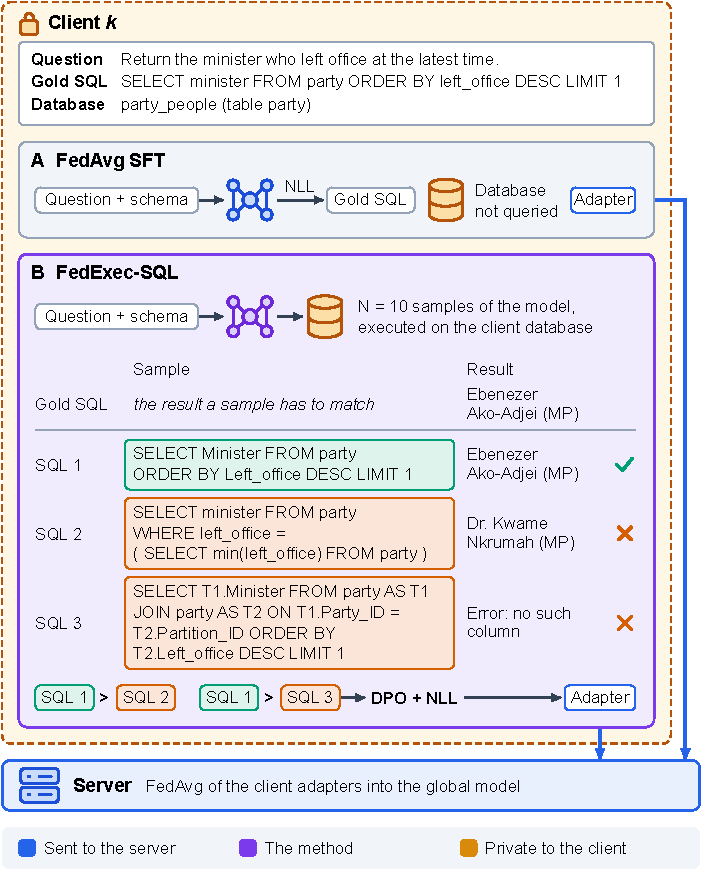
\includegraphics{figures/fig_idea.pdf}
\caption{Local supervision on one BIRD training question (database \texttt{language\_corpus}) within the dashed boundary of client~$k$. \panel{a}~In federated averaging with supervised fine-tuning (FedAvg SFT), the prompt (schema, question, and evidence) and gold SQL query define the negative log-likelihood (NLL) loss, and the database is not queried. \panel{b}~In the first preference round of \method{} (from the global model after \setting{rounds.warmup} warm-up rounds, temperature~\setting{pref.t}, at most \setting{pref.tokens} new tokens), executing $N = {}$\setting{pref.samples} samples on \texttt{language\_corpus} yields eight correct samples, one incorrect result, and one execution error. The table displays the samples of the $M = {}$\setting{pref.pairs} preference pairs built for this question beside the gold execution result, where two distinct correct samples with identical SQL text (first row) are paired against the incorrect result and the execution error (second and third rows) under the direct preference optimization (DPO) plus NLL loss.}
\label{fig:idea}
\end{figure}

Executing queries sampled from the model on the client's database and comparing their results with that of the gold SQL query turns the one gold SQL query of a question into several labeled queries of the model's own, correct and incorrect (Fig.~\ref{fig:idea}, Section~\ref{sec:supervision}). Only the client can produce these labels, since only the client holds the database.

We propose \method, a federated learning framework for Text-to-SQL that trains on this execution-derived supervision. It has four components (Section~\ref{sec:overview}, Fig.~\ref{fig:overview}). \textit{Supervised warm-up} runs the first rounds as rounds of FedAvg SFT on the gold SQL queries, so that fewer training questions have only incorrect samples. In each of the following preference rounds, \textit{client-side execution labeling} samples several queries per question from the current global model and labels each by executing it on the client's database against the result of the gold SQL query. \textit{On-policy pair construction} forms preference pairs of a correct and an incorrect sample from these labels. The \textit{preference objective} trains the adapter with a DPO term, whose reference model is the current global model, plus an NLL term on the correct sample of each pair, and the server averages the adapters by the pair counts of the clients. A preference round thus renews the pairs and the reference model together. In every round, a client sends the same adapter as in FedAvg SFT, and a preference round adds client computation for sampling, labeling and training.

We evaluate \method{} with the SLM \setting{model} (\setting{model.size} parameters)~\cite{hui2024qwen25coder} on BIRD~\cite{li2023bird} and Spider~\cite{yu2018spider}, with \fact{split.bird.a0.1.k5.clients} clients that all take part in every round and hold disjoint sets of databases (Section~\ref{sec:fed-setups}). At \setting{rounds.total} rounds, \method{} reaches \ex{bird}{k2}{4}\% execution accuracy (EX) on BIRD dev against \ex{bird}{fedavg}{4}\% for FedAvg SFT, a gain of \gap{bird}{fedavg}{4}{k2}{4} points, and \ex{spider}{k2}{4}\% on Spider test against \ex{spider}{fedavg}{4}\%, a gain of \gap{spider}{fedavg}{4}{k2}{4} points. Further rounds of FedAvg SFT do not close the gap: its highest EX on BIRD dev, \ex{bird}{fedavg}{3}\% after the third round, is \gap{bird}{fedavg}{3}{k2}{4} points below \method. On BIRD dev, \method{} is also above FedDPO run on the first execution-labeled pairs of \method, with the pairs and the reference model of that round fixed and the DPO loss alone, by \gap{bird}{feddpo}{4}{k2}{4} EX points and \tsgap{bird}{feddpo}{4}{k2}{4} points of test-suite accuracy (TS). Against FedAvg SFT, execution errors fall by about half on both benchmarks, from \nerr{bird}{fedavg}{4} to \nerr{bird}{k2}{4} on BIRD dev, while incorrect results do not fall. With the settings of the preference rounds held equal, \method{} is \gap{bird}{k2}{4}{rft}{4} EX points above the variant trained without the preference term on BIRD dev (Section~\ref{sec:ablation}). Each difference named in this paragraph is significant under the test of Section~\ref{sec:stat-test}.

In summary, we make four contributions:
\begin{itemize}
\item We identify the databases of the clients as a source of execution-derived supervision that federated fine-tuning leaves unused, and introduce, to our knowledge, the first federated training method for Text-to-SQL that uses it (Sections~\ref{sec:rel-fedsql} and~\ref{sec:supervision}).
\item We design \method{} with supervised warm-up, client-side execution labeling, on-policy pair construction and a preference objective of a DPO term and an NLL term (Section~\ref{sec:method}). Each preference round renews the pairs and the reference model together, and only the LoRA adapter and its integer weight leave a client.
\item We show that, at the same number of rounds, \method{} is above FedAvg SFT on BIRD dev and Spider test with about half as many execution errors, and that on BIRD dev it is above FedDPO run on the first execution-labeled pairs of \method under EX and TS (Sections~\ref{sec:main} and~\ref{sec:analysis}). We measure what each component adds and what a client pays in computation (Sections~\ref{sec:ablation} and~\ref{sec:cost}).
\item We release our code, federated client splits, and evaluation predictions for every row of the tables.
\end{itemize}

\section{Related work}\label{sec:related}

\subsection{Fine-tuned open models for Text-to-SQL}\label{sec:rel-slm}

Open models fine-tuned for Text-to-SQL differ above all in what they are
trained on. CodeS~\cite{li2024codes} continues the pre-training of
StarCoder models of 1B to 15B parameters on a SQL-centric corpus and then
fine-tunes all their parameters on the training set of each benchmark.
OmniSQL~\cite{li2025omnisql} fine-tunes Qwen2.5-Coder-Instruct models of
7B, 14B and 32B parameters on SynSQL-2.5M, about 2.5 million synthetic
samples, together with the training sets of Spider and BIRD. SLM-SQL~\cite{sheng2025slmsql} studies the range of
model sizes of this paper, 0.5B to 1.5B. It fine-tunes on 916K synthetic
samples, trains further with Group Relative Policy Optimization (GRPO) on
BIRD train with a reward for a correct execution result, and at inference
groups 64 samples by their execution results and votes, whereas our
models train on the benchmark training sets alone and decode greedily.
SPFT-SQL~\cite{zhang2025spftsql} synthesizes SQL queries from templates
over the training databases, checks the outputs of the fine-tuned model
by execution against them, and then fine-tunes the model in self-play
against a weaker opponent model. SKT-SQL~\cite{yi2025sktsql} guides
smaller-scale language models with a generated SQL skeleton. Each of
these models is trained on data held in one place.

\subsection{Preference optimization and execution feedback}\label{sec:rel-pref}

DPO~\cite{rafailov2023dpo} trains a model on pairs of a preferred and a
dispreferred response without a reward model or reinforcement learning,
through the negative log-sigmoid of the difference of their log-ratios
under the trained model and a reference model, multiplied by $\beta$,
the scale of the preference term. The reference model is the SFT model
when one is available.

Execution first served Text-to-SQL at inference: LEVER~\cite{ni2023lever}
trains a verifier on the question, a sampled program and its execution
result to rerank samples, and GradeSQL~\cite{tritto2026gradesql} trains
reward models on candidates labeled by execution to select among them,
and neither trains the model that generates the queries. In training,
Think2SQL~\cite{papicchio2025think2sql} and
Arctic-Text2SQL-R1~\cite{yao2026arctic} apply GRPO with rewards computed
by execution, partial scores of the result in Think2SQL, and 1 for a
matching result and 0.1 for an executable query in Arctic-Text2SQL-R1.
Liu et al.~\cite{liu2025cotdpo} and ExCoT~\cite{zhai2025excot} label
preference pairs by execution. Liu et al.\ sample 16 queries per BIRD
training question from the SFT model, pair a correct with an incorrect
sample, and train with DPO against the SFT model as reference. With
SQL-only outputs, DPO lowers BIRD dev EX for 6 of their 10 models of
6.7B to 15B parameters under greedy decoding and majority voting and
raises it for all ten under Pass@1, and with synthesized chains of
thought it raises EX for all ten. ExCoT trains Llama-3.1 70B and
Qwen-2.5-Coder 32B in one DPO round on pairs of GPT-4o outputs and then
in on-policy rounds on new samples of the model, labeled again by
execution.

A likelihood term on the preferred response beside the DPO term has
published results in both directions. Iterative reasoning preference
optimization (Iterative RPO)~\cite{pang2024irpo} samples chains of
thought from the current model, pairs correct with incorrect final
answers, and trains with the DPO term plus a
length-normalized NLL term on the preferred response, with the model of
the previous iteration as reference. After one round on GSM8K, it
reaches 73.1 with the NLL term and 61.8 with DPO alone, and
CodeLutra~\cite{tao2024codelutra} reports 76.6 on Spider with its full
loss against 17.2 with the DPO term alone. Liu et al.\ report a limited gain
from an added SFT term on SQL-only outputs, 58.8 to 60.0 with
Qwen2.5-7B-Instruct, and Lanchantin et al.~\cite{lanchantin2025bridging}
report no benefit from an added NLL term.

CodeLutra is the closest work. From one training set at one site, it
samples ten outputs per question from the current model, labels each SQL
query by comparing its execution result with that of the gold query, and
forms $K$ pairs per question of a correct and a failed sample.
It trains with the DPO term, whose reference model is the model of the
previous iteration, plus $\lambda$ times the log-likelihood of the
correct sample, over four iterations. With Llama-3-8B, its Spider EX
reaches 76.6 at the third iteration against 67.9 for SFT. CodeLutra thus
runs the loop of sampling, execution labels and DPO with an NLL term
centrally, by one holder of the data. In \method, the labels are
computed at each client on databases that the server never sees, a
federated round is the re-sampling step, and the global model of the
round is the reference model of every client.

\subsection{Federated fine-tuning of language models}\label{sec:rel-fed}

FederatedScope-LLM~\cite{kuang2024fsllm} and
OpenFedLLM~\cite{ye2024openfedllm} provide federated fine-tuning of LLMs
with LoRA and other parameter-efficient methods, run FedAvg among other
algorithms, and include code tasks. In federated SFT, a client trains on
the responses of its dataset, not on outputs of the model. OpenFedLLM
also introduces FedDPO, in which every client keeps its own preference
dataset and trains with the DPO loss alone against a reference model fixed
throughout the federated process. Its runs train
Wizard-Vicuna-7B-Uncensored with LoRA of rank 8 on UltraFeedback and
HH-RLHF, with five clients of which two take part in each round, and no
step that constructs pairs again is described. In FedBis and
FedBiscuit~\cite{wu2025fedbiscuit}, clients train binary selectors on
their preference data, and the server aggregates the selectors, labels
with them pairs that its initial model generates once, and trains the
LLM with DPO. In federated reinforcement learning with verifiable
rewards, a client samples from the current model and trains with GRPO on
a reward for correct answers: PubSwap~\cite{nayak2026pubswap} on math
and medical questions, with LoRA adapters averaged at the server, and
Fed-GRPO~\cite{guo2026fedgrpo} on math and code, with clients weighted
by the standard deviation of their rewards. These two methods use a
policy-gradient objective and no pairs, and none of the works of this
subsection addresses Text-to-SQL.

\subsection{Federated semantic parsing and Text-to-SQL}\label{sec:rel-fedsql}

\begin{table}[!ht]
\caption{Methods closest to \method. ``Labels from execution'': a sample
is labeled by executing it and comparing its result with the gold
result. ``Preference pairs'': where the pairs of the preference
objective come from.}\label{tab:related}
\footnotesize
\setlength{\tabcolsep}{3pt}
\begin{tabular}{@{}lccccl@{}}
\toprule
Method & Federated & Text-to-SQL &
\begin{tabular}[c]{@{}c@{}}Labels from\\ execution\end{tabular} &
\begin{tabular}[c]{@{}c@{}}Trains on the\\ model's own outputs\end{tabular} &
Preference pairs \\
\midrule
Zhang et al.~\cite{zhang2023fl4sp} & Yes & Yes & No & No & Not applicable \\
FedDPO~\cite{ye2024openfedllm} & Yes & No & No & No & From a dataset\textsuperscript{a} \\
PubSwap~\cite{nayak2026pubswap} & Yes & No & Answer check\textsuperscript{b} & Yes & Not applicable \\
Fed-GRPO~\cite{guo2026fedgrpo} & Yes & No & Answer check\textsuperscript{b} & Yes & Not applicable \\
Liu et al.~\cite{liu2025cotdpo} & No & Yes & Yes & Yes & Once, from the model's outputs \\
ExCoT~\cite{zhai2025excot} & No & Yes & Yes & Yes\textsuperscript{c} & Anew each round\textsuperscript{c} \\
CodeLutra~\cite{tao2024codelutra} & No & Yes & Yes & Yes & Anew each round \\
\midrule
\method{} (ours) & Yes & Yes & Yes & Yes & Anew each round \\
\bottomrule
\end{tabular}

\smallskip
\begin{minipage}{\linewidth}
\textsuperscript{a}~Every client keeps its own preference dataset, and
no step that constructs pairs again is described.\par
\textsuperscript{b}~The reward checks whether the answer to a math,
medical (PubSwap) or code (Fed-GRPO) task is correct, and no SQL query
is executed.\par
\textsuperscript{c}~Only in the on-policy rounds: the first DPO round
trains on pairs of GPT-4o outputs.
\end{minipage}
\end{table}

Zhang et al.~\cite{zhang2023fl4sp} study federated Text-to-SQL with
eight single-domain datasets as clients. They fine-tune T5-base with
FedAvg, FedOPT and FedProx on the gold SQL queries of each client,
weight the clients by their data size and the reduction of their
training loss, and score predictions by exact match with the gold SQL
query, without executing any query. Their best federated variant reaches
62.55 macro-averaged exact match against 70.32 for centralized training.
KGRFL~\cite{xu2024kgrfl}, which converts questions into SPARQL, fuses
the client models with a strategy based on reinforcement learning. To
our knowledge, no earlier method for federated training of Text-to-SQL
models uses the databases of the clients for execution labels.
Table~\ref{tab:related} sets the closest methods beside \method, which
Section~\ref{sec:method} presents.

\section{Method}\label{sec:method}

In \method, the model learns from the execution of its own sampled queries
on the client databases. In each preference round, a client samples SQL
queries from the current global model, executes them on its databases,
labels them by comparison with the execution result of the gold SQL query
and trains on pairs of a correct and an incorrect sample of the same
question.

\subsection{Problem Formulation}\label{sec:formulation}

We consider $K$ clients. Client $k$ holds a training set $\mathcal{D}_k$
of $n_k$ elements $(q, d, y^\star)$, each consisting of a question $q$, the
database $d$ on which it is posed and its gold SQL query $y^\star$. None
of them leaves the client. The clients jointly train one model: the
pretrained model is frozen, and a LoRA adapter $\theta$~\cite{hu2022lora}
is the only set of parameters that is trained, communicated and
aggregated. We write $\pi_\theta$ for the model with adapter $\theta$. The
prompt $x$ contains $q$ and the schema of $d$ as \texttt{CREATE TABLE}
statements. On Spider each statement is followed by up to three rows of
its table, and on BIRD the prompt adds the external knowledge that the
benchmark attaches to the question (Fig.~\ref{fig:prompt},
Appendix~\ref{app:prompt}). The same prompt serves training, sampling and
evaluation. Training runs for $T$ rounds, all $K$ clients participating
in each. In round $t$, the server sends the global adapter
$\theta^{t-1}$, client $k$ obtains $\theta_k^{t}$ by local training from
$\theta^{t-1}$ with a newly initialized optimizer, and the server
aggregates the client adapters into $\theta^{t}$.

FedAvg SFT~\cite{mcmahan2017fedavg,ye2024openfedllm} trains the adapter
on the gold SQL queries. Client $k$ minimizes the token-averaged NLL of
the gold SQL query,
\begin{equation}
  \mathcal{L}_k^{\mathrm{SFT}}(\theta) = \frac{1}{n_k}
    \sum_{(q, d, y^\star) \in \mathcal{D}_k}
    -\frac{1}{\lvert y^\star \rvert} \log \pi_\theta(y^\star \mid x),
  \label{eq:sft}
\end{equation}
and uploads $\theta_k^{t}$ together with $n_k$. The server averages the
adapters with weights proportional to the numbers of questions:
\begin{equation}
  \theta^{t} = \sum_{k=1}^{K} w_k \, \theta_k^{t},
  \qquad
  w_k = \frac{n_k}{\sum_{j=1}^{K} n_j}.
  \label{eq:aggregation}
\end{equation}
In Eq.~\eqref{eq:sft}, the gold SQL query is the only target and the
database enters only as text of the prompt. During local
training the model generates no query, so no loss term is computed on a
query of its own. Neither the gold SQL query nor a query of the model is
executed, no execution result enters the loss, and nothing identifies
which of the model's queries are incorrect.

\subsection{Execution-Derived Supervision}\label{sec:supervision}

A SQL query is verifiable by execution. Let $\mathrm{exec}(y, d)$ denote
the execution result of a query $y$ on the database $d$. For an element
$(q, d, y^\star)$, a query $y$ that the model generates for $q$ can be
labeled correct or incorrect by comparing $\mathrm{exec}(y, d)$ with
$\mathrm{exec}(y^\star, d)$. Execution thus turns the single gold SQL
query of a question into many labeled queries of the model's own,
incorrect ones among them. We refer to the training signal that these
labels provide as execution-derived supervision. It requires both $d$
and $y^\star$ and can therefore be computed only at the client.

On BIRD, this signal is available for most training questions. In the
BIRD setup of Section~\ref{sec:fed-setups}, \setting{pref.samples}
samples per question from the global model after
\setting{rounds.warmup} rounds of FedAvg SFT (Section~\ref{sec:labeling})
include both a correct and an incorrect sample for
\fact{cost.bird.pref1.paired_pct}\% of all
\fact{cost.bird.pref1.questions} training questions of the clients.

\subsection{Framework Overview}\label{sec:overview}

\begin{figure}[!t]
\centering
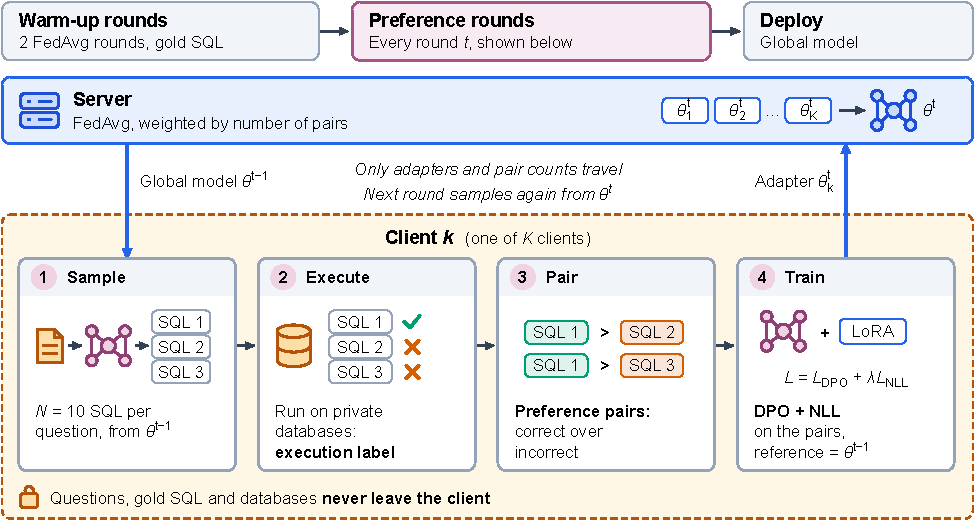
\includegraphics{figures/fig_method_overview.pdf}
\caption{Overview of \method. On the arrows, ``Global model
$\theta^{t-1}$'' denotes the global adapter, and ``count'' is $n_k$ in a
warm-up round and $\lvert\mathcal{P}_k^{t}\rvert$ in a preference round.
In step~1 and step~4, $\theta^{t-1}$ stands for the model
$\pi_{\theta^{t-1}}$, which is $\pi_{\mathrm{ref}}$ in
Eq.~\eqref{eq:logratio}. Step~1 shows the default setting
$N = {}$\setting{pref.samples}. In step~4, $L_{\mathrm{DPO}}$ and
$L_{\mathrm{NLL}}$ are the preference term and the NLL term of
Eq.~\eqref{eq:loss}.}
\label{fig:overview}
\end{figure}

We propose \method, a federated learning framework for Text-to-SQL that
trains on execution-derived supervision. It consists of four components
and an aggregation rule, organized into two kinds of round
(Fig.~\ref{fig:overview}, Algorithm~\ref{alg:method}) that differ in the
role of the gold SQL query. In the warm-up rounds $1, \dots, T_w$ it is
the training target, whereas in the preference rounds
$T_w + 1, \dots, T$ it is executed to produce the execution labels and
is not a training target. Every round ends with federated averaging of
the adapters. Supervised warm-up (Section~\ref{sec:warmup}) consists of
the warm-up rounds, which are rounds of FedAvg SFT. The other three
components make up a preference round: client-side execution labeling
(Section~\ref{sec:labeling}) samples $N$ queries per question from the
current global model and labels them by execution, on-policy pair
construction (Section~\ref{sec:pairs}) forms $M$ preference pairs per
question from these samples, and the preference objective
(Section~\ref{sec:objective}) trains the adapter on the pairs, with the
current global model as reference model. By default,
$T = {}$\setting{rounds.total}, $T_w = {}$\setting{rounds.warmup},
$N = {}$\setting{pref.samples} and $M = {}$\setting{pref.pairs}, with
\setting{sft.epochs} local epoch per warm-up round and
\setting{pref.epochs} per preference round. Table~\ref{tab:settings} in
Appendix~\ref{app:settings} lists the remaining settings, and
Section~\ref{sec:main} reports the resulting gain over FedAvg SFT
(Table~\ref{tab:main}).

\begin{algorithm}[t]
\caption{\method}\label{alg:method}
\begin{algorithmic}[1]
\Require training sets $\{\mathcal{D}_k\}_{k=1}^{K}$, pretrained model,
  $T$, $T_w$, $N$, $M$, $\beta$, $\lambda$
\Ensure global adapter $\theta^{T}$
\State initialize the adapter $\theta^{0}$
\For{$t = 1, \dots, T$}
  \State the server sends $\theta^{t-1}$ to all $K$ clients
  \ForAll{clients $k = 1, \dots, K$ in parallel}
    \If{$t \le T_w$} \Comment{warm-up round}
      \State $\theta_k^{t} \gets$ local training from $\theta^{t-1}$ on
        $\mathcal{D}_k$ with the loss of Eq.~\eqref{eq:sft}
      \State upload $\theta_k^{t}$ and $n_k$
    \Else \Comment{preference round}
      \State sample $N$ queries from $\pi_{\theta^{t-1}}(\cdot \mid x)$
        for each $(q, d, y^\star) \in \mathcal{D}_k$
      \State label the samples by comparing $\mathrm{exec}(y, d)$
        with $\mathrm{exec}(y^\star, d)$
        (Section~\ref{sec:labeling})
      \State $\mathcal{P}_k^{t} \gets$ $M$ pairs $(y^{+}, y^{-})$ for
        each question that yields pairs (Section~\ref{sec:pairs})
      \If{$\mathcal{P}_k^{t} \neq \emptyset$}
        \Comment{otherwise no update, $w_k = 0$}
        \State $\theta_k^{t} \gets$ local training from $\theta^{t-1}$
          on $\mathcal{P}_k^{t}$ with the loss of Eq.~\eqref{eq:loss},
          $\pi_{\mathrm{ref}} = \pi_{\theta^{t-1}}$
        \State upload $\theta_k^{t}$ and $\lvert\mathcal{P}_k^{t}\rvert$
      \EndIf
    \EndIf
  \EndFor
  \State $\theta^{t} \gets \sum_{k=1}^{K} w_k \, \theta_k^{t}$, with
    $w_k \propto n_k$ if $t \le T_w$ and
    $w_k \propto \lvert\mathcal{P}_k^{t}\rvert$ otherwise
\EndFor
\State \Return $\theta^{T}$
\end{algorithmic}
\end{algorithm}

\subsection{Supervised Warm-Up}\label{sec:warmup}

A preference pair needs a correct sample, and a question whose labeled
samples are all incorrect yields none. Measured as in
Section~\ref{sec:supervision}, this is the case for
\fact{warmup.bird.k0.no_correct} of the
\fact{cost.bird.pref1.questions} BIRD training questions under the
pretrained model. We reduce their number by supervised warm-up: in each
of the first $T_w$ rounds, client $k$ minimizes Eq.~\eqref{eq:sft} over
$\mathcal{D}_k$ and the server aggregates by
Eq.~\eqref{eq:aggregation}, as in FedAvg SFT. After
\setting{rounds.warmup} warm-up rounds, the labeled samples are all
incorrect for \fact{warmup.bird.k2.no_correct} questions. Neither count
includes the questions whose gold SQL query fails to execute or exceeds
the time limit, as their samples receive no label
(Section~\ref{sec:labeling}).

Warm-up is a setting of the framework, not a precondition of the
preference rounds. The adapter $\theta^{0}$
has the standard LoRA initialization, under which $\pi_{\theta^{0}}$ is
the pretrained model. With $T_w = 0$, the first round of
Algorithm~\ref{alg:method} therefore samples from the pretrained model,
which already yields preference pairs, and uses it as reference model.
Section~\ref{sec:ablation} examines the effect of $T_w$ on accuracy.

\subsection{Client-Side Execution Labeling}\label{sec:labeling}

In preference round $t$, client $k$ samples $N$ queries for each element
of $\mathcal{D}_k$ from $\pi_{\theta^{t-1}}(\cdot \mid x)$ at
temperature \setting{pref.t}, without nucleus or top-$k$ truncation and
with at most \setting{pref.tokens} new tokens per sample. It executes
each sample $y$ and, once per question, the gold SQL query $y^\star$ on
$d$, under the time limit of the benchmark's evaluation
(Section~\ref{sec:setup}). The execution label of $y$ is correct if
$\mathrm{exec}(y, d) = \mathrm{exec}(y^\star, d)$ under the comparison of
the evaluation metric, and incorrect otherwise. A sample that fails to
execute, reaches the time limit while it runs or contains no query is
therefore incorrect.

A sample has no label when its result is never compared with the gold
result. This is the case when the sample is cut at the token limit and
not executed, when the time limit is reached after
the sample has completed but before the comparison
(Section~\ref{sec:setup}), and when the gold SQL query fails to execute
or exceeds the time limit, which leaves the whole question without
labels.

\subsection{On-Policy Preference Pair Construction}\label{sec:pairs}

We construct the preference pairs $\mathcal{P}_k^{t}$ of client $k$ anew
in every preference round $t$, from that round's labeled samples.
FedDPO~\cite{ye2024openfedllm} instead trains each client on a fixed
preference dataset whose responses are not outputs of the model under
training. A question yields
pairs when it has at least one correct and one incorrect sample and some
table of its database contains a row. On a database without rows,
queries of different meaning return the same result, and a sample that
executes can match the gold result whether or not it is correct. We
exclude the questions on such a database, although their samples are
labeled (Section~\ref{sec:fed-setups}).

For each question that yields pairs, we draw $M$ samples uniformly from
its correct samples and, independently, $M$ from its incorrect samples.
Each draw is without replacement when the question has at least $M$
samples of that label and with replacement otherwise, and identical
queries among the samples are not merged. Pairing the two draws in order
gives $M$ pairs $(y^{+}, y^{-})$ per question, so that
$\lvert\mathcal{P}_k^{t}\rvert$ is $M$ times the number of questions of
client $k$ that yield pairs. We draw a fixed number of pairs per
question, rather than all combinations of its correct and incorrect
samples, so that every question that yields pairs carries the same
weight in the local objective. One local epoch runs over $M$ pairs of
each such question, and $M$ thereby sets the length of local training
per question.

With pairs constructed in every round, one iteration of preference
optimization, sampling from the current model and training on its
labeled samples, coincides with one communication round, and the
incorrect queries of each new global model are identified anew at no
additional communication. A question without pairs contributes to
neither term of the objective in that round, the NLL term included, and
like every question it is sampled again in the next preference round.
Section~\ref{sec:ablation} compares this construction with the pairs and
the reference model of the first preference round, and with the gold SQL
query in place of a missing correct sample.

\subsection{Preference Objective and Aggregation}\label{sec:objective}

In a preference round, client $k$ minimizes the mean over
$\mathcal{P}_k^{t}$ of a loss that combines a preference term, the DPO
loss~\cite{rafailov2023dpo}, with an NLL term on the correct
sample~\cite{pang2024irpo,tao2024codelutra}. For a pair
$(y^{+}, y^{-})$ of a question with prompt $x$,
\begin{equation}
  m_\theta = \beta \left[
    \log \frac{\pi_\theta(y^{+} \mid x)}{\pi_{\mathrm{ref}}(y^{+} \mid x)}
    - \log \frac{\pi_\theta(y^{-} \mid x)}{\pi_{\mathrm{ref}}(y^{-} \mid x)}
  \right],
  \label{eq:logratio}
\end{equation}
\begin{equation}
  \ell(\theta) = -\log \sigma(m_\theta)
    - \frac{\lambda}{\lvert y^{+} \rvert} \log \pi_\theta(y^{+} \mid x),
  \label{eq:loss}
\end{equation}
where $\pi_{\mathrm{ref}} = \pi_{\theta^{t-1}}$ is the reference model,
$\sigma$ the logistic function, $\beta$ the scale of the preference term
and $\lambda$ the weight of the NLL term. We write Eq.~\eqref{eq:loss}
as $\ell = L_{\mathrm{DPO}} + \lambda L_{\mathrm{NLL}}$, with the
preference term $L_{\mathrm{DPO}}$ and the NLL term $L_{\mathrm{NLL}}$.
By default, $\beta = {}$\setting{pref.beta} and
$\lambda = {}$\setting{pref.nll}. The log-likelihoods in
Eq.~\eqref{eq:logratio} are sums over tokens, whereas $L_{\mathrm{NLL}}$,
like Eq.~\eqref{eq:sft}, is a token mean.

We reset the reference model to the global model at the start of each
preference round, whereas FedDPO keeps one reference model for the whole
federated process. Local training starts from $\theta^{t-1}$, that is,
from the reference model, so $m_\theta = 0$ for every pair when local
training begins. The reference model also generated the samples of the round, so
the log-ratios of Eq.~\eqref{eq:logratio} are taken relative to the
model that generated both samples of each pair.

The preference term raises the likelihood of the correct sample relative
to that of the incorrect one and is the only term that uses the
incorrect sample. It constrains only a difference of log-ratios: it is
invariant to a common shift of $\log \pi_\theta(y^{+} \mid x)$ and
$\log \pi_\theta(y^{-} \mid x)$ and can decrease while both likelihoods
decrease. We add the NLL term, which the loss of FedDPO does not
contain, to act on what this difference leaves undetermined: it raises
the log-likelihood of the correct sample itself.
Section~\ref{sec:ablation} removes each term in turn
(Table~\ref{tab:ablation}).

In a preference round, a client uploads its adapter
(\setting{adapter.mb}) and one integer, its pair count
$\lvert\mathcal{P}_k^{t}\rvert$, in place of its question count $n_k$ in
a warm-up round. Communication per round is thus the same in both kinds
of round. Samples, execution results, execution labels and preference
pairs remain at the client. We weight the average by the pair counts:
the server aggregates by Eq.~\eqref{eq:aggregation} with
$\lvert\mathcal{P}_k^{t}\rvert$ in place of $n_k$, since federated
averaging weights a client by its number of local training examples,
which in a preference round are its pairs. A client without pairs
performs no local training, sends no update and has weight zero.
Section~\ref{sec:ablation} examines the choice of the weights.

A preference round differs in cost from a warm-up round only in client
computation. In place of an epoch over $\mathcal{D}_k$, the client
generates $N n_k$ samples, executes them and performs an epoch over
$\mathcal{P}_k^{t}$. It computes the log-likelihoods of the reference
model once per pair before the first update, so the epoch evaluates only
the model under training. Section~\ref{sec:cost} reports the measured
times (Table~\ref{tab:cost}).

\section{Experimental setup}\label{sec:setup}

% To be written from the brief of this section.

\section{Results and analysis}\label{sec:results}

\subsection{Main results}\label{sec:main}

\begin{table}[!ht]
\caption{EX (\%) on BIRD dev and Spider test, overall and at each
difficulty level of the benchmark. Federated models are after
\setting{rounds.total} rounds, and centralized SFT after
\setting{central.epochs} epochs. Models marked ``second seed'' repeat
the training with another seed. $\Delta$ and $p$ compare each model with
FedAvg SFT of the same block. The $p$ is that of the exact McNemar test after the Holm correction, and
an asterisk marks a significant difference
(Section~\ref{sec:stat-test}). Bold marks the
highest value of each column within a block.}\label{tab:main}
\footnotesize
%% Written by tools/paper_numbers.py. Do not edit.
\setlength{\tabcolsep}{3.5pt}%
\begin{tabular}{@{}lrrrrrrl@{}}
\toprule
BIRD dev & EX & Simple & Moderate & Challenging &  & $\Delta$ & $p$ \\
\midrule
No training & 29.47 & 35.89 & 20.47 & 17.24 &  & $-$13.10 & $8.4\times10^{-27}$\textsuperscript{*} \\
Local SFT & -- & -- & -- & -- &  & -- & -- \\
Centralized SFT & -- & -- & -- & -- &  & -- & -- \\
FedAvg SFT & 42.57 & 51.35 & 29.96 & 26.90 &  &  &  \\
FedDPO & 45.50 & 52.54 & 35.99 & 31.03 &  & +2.93 & 0.014\textsuperscript{*} \\
\method & \textbf{48.76} & \textbf{56.00} & \textbf{39.66} & \textbf{31.72} &  & +6.19 & $2.3\times10^{-10}$\textsuperscript{*} \\
\method{} against centralized SFT &  &  &  &  &  & -- & -- \\
\midrule
Spider test & EX & Easy & Medium & Hard & Extra & $\Delta$ & $p$ \\
\midrule
No training & 68.05 & 87.45 & 71.41 & 59.18 & 45.94 & $-$6.66 & $8.6\times10^{-15}$\textsuperscript{*} \\
Centralized SFT & 75.03 & 91.06 & 78.30 & 67.17 & 56.30 & +0.32 & 0.69 \\
FedAvg SFT & 74.71 & 90.64 & 78.18 & 66.74 & 55.74 &  &  \\
FedDPO & -- & -- & -- & -- & -- & -- & -- \\
\method & \textbf{78.20} & \textbf{91.91} & \textbf{81.91} & \textbf{71.06} & \textbf{60.50} & +3.49 & $2.6\times10^{-6}$\textsuperscript{*} \\
\method{} against centralized SFT &  &  &  &  &  & +3.17 & $7.1\times10^{-5}$\textsuperscript{*} \\
\bottomrule
\end{tabular}

\end{table}

At \setting{rounds.total} rounds, \method{} is significantly above
FedAvg SFT on both benchmarks, by \gap{bird}{fedavg}{4}{k2}{4} EX points
on BIRD dev and \gap{spider}{fedavg}{4}{k2}{4} on Spider test, and it is
higher at every difficulty level, most of all on the moderate questions
of BIRD dev and on the extra-hard questions of Spider test
(Table~\ref{tab:main}). It is also significantly above FedDPO on BIRD
dev and centralized SFT on Spider test, and further rounds of FedAvg SFT
do not close the gap (Fig.~\ref{fig:rounds}).

\begin{figure}[!t]
\centering
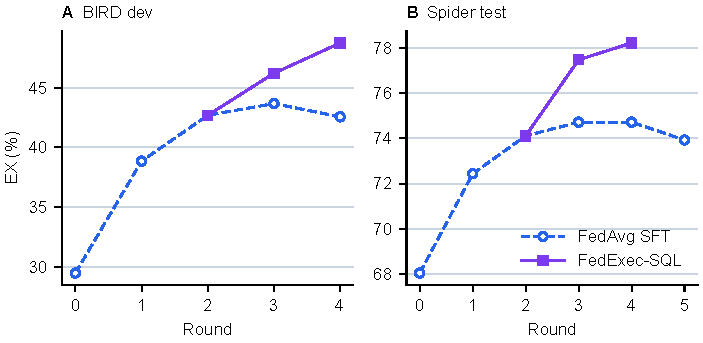
\includegraphics{figures/fig_rounds_cmc.pdf}
\caption{EX by round on \panel{a} BIRD dev and \panel{b} Spider test.
Round~0 is the pretrained model. \method{} continues from the FedAvg SFT
model of round~\setting{rounds.warmup}, and FedAvg SFT has a fifth round
on Spider test.}
\label{fig:rounds}
\end{figure}

FedAvg SFT does not improve after its third round on either benchmark.
On BIRD dev, its fourth round changes EX by
\gain{bird}{fedavg}{3}{fedavg}{4} points
($p = {}$\padj{bird}{fedavg}{3}{fedavg}{4}), and its highest EX,
\ex{bird}{fedavg}{3}\% after the third round, is
\gap{bird}{fedavg}{3}{k2}{4} points below \method{}
($p = {}$\padj{bird}{fedavg}{3}{k2}{4}). On Spider test, it stays at
\ex{spider}{fedavg}{3}\% after its third and fourth rounds and reaches
\ex{spider}{fedavg}{5}\% after a fifth
($p = {}$\padj{spider}{fedavg}{4}{fedavg}{5} against the fourth). With
this fifth round, FedAvg SFT uses more GPU time than \method{} does in
four (Section~\ref{sec:cost}), and \method{} is
\gap{spider}{fedavg}{5}{k2}{4} points above it
($p = {}$\padj{spider}{fedavg}{5}{k2}{4}).

From the same model after \setting{rounds.warmup} rounds, one preference
round adds more than one further round of FedAvg SFT, significantly so on
Spider test (Fig.~\ref{fig:rounds}). On BIRD dev, the preference round
adds \gap{bird}{fedavg}{2}{k2}{3} points
($p = {}$\padj{bird}{fedavg}{2}{k2}{3}) and the FedAvg SFT round
\gap{bird}{fedavg}{2}{fedavg}{3} ($p = {}$\padj{bird}{fedavg}{2}{fedavg}{3}),
and the two models after three rounds differ by
\gap{bird}{fedavg}{3}{k2}{3} points ($p = {}$\padj{bird}{fedavg}{3}{k2}{3}).
On Spider test, the two steps are \gap{spider}{fedavg}{2}{k2}{3}
($p = {}$\padj{spider}{fedavg}{2}{k2}{3}) and
\gap{spider}{fedavg}{2}{fedavg}{3} points
($p = {}$\padj{spider}{fedavg}{2}{fedavg}{3}), and the two models after
three rounds differ by \gap{spider}{fedavg}{3}{k2}{3} points
($p = {}$\padj{spider}{fedavg}{3}{k2}{3}). The preference round takes
more GPU time than the FedAvg SFT round in both setups
(Section~\ref{sec:cost}).

On Spider test, centralized SFT after \setting{central.epochs} epochs
does not differ significantly from FedAvg SFT, and \method{} is \gap{spider}{central}{3}{k2}{4} points above
it ($p = {}$\padj{spider}{central}{3}{k2}{4}).

FedDPO, trained on the fixed execution-labeled pairs of the first
preference round of \method, is \gap{bird}{feddpo}{4}{k2}{4} EX points
($p = {}$\padj{bird}{feddpo}{4}{k2}{4}) and \tsgap{bird}{feddpo}{4}{k2}{4}
TS points ($p = {}$\tspadj{bird}{feddpo}{4}{k2}{4}) below \method{} on
BIRD dev at \setting{rounds.total} rounds, where its TS is
\ts{bird}{feddpo}{4}\%. After the first of the two preference
rounds, FedDPO is below \method{} by a difference that is not
significant, and its second round adds \gain{bird}{feddpo}{3}{feddpo}{4}
points ($p = {}$\padj{bird}{feddpo}{3}{feddpo}{4}), less than the second
preference round of \method{} adds (Section~\ref{sec:ablation}). Against
FedAvg SFT, FedDPO is significantly higher under EX and does not differ
significantly under TS (\tsgain{bird}{fedavg}{4}{feddpo}{4} points,
$p = {}$\tspadj{bird}{fedavg}{4}{feddpo}{4}). Trained on these pairs,
FedDPO differs from \method{} in two components, the renewal of the pairs
and the reference model and the NLL term, and
Section~\ref{sec:ablation} gives the effect of each.

\subsection{Analysis of the predictions}\label{sec:analysis}

The gain over FedAvg SFT comes with about half as many execution errors,
while incorrect results do not fall (Fig.~\ref{fig:errors}). An
execution error is an incorrect prediction that fails to execute,
reaches the time limit or is cut at the token limit, and an incorrect
result is one that executes and returns another result than the gold
SQL query. At \setting{rounds.total} rounds, execution errors go from
\nerr{bird}{fedavg}{4} with FedAvg SFT to \nerr{bird}{k2}{4} with
\method{} on BIRD dev ($p = {}$\errpadj{bird}{fedavg}{4}{k2}{4}) and from
\nerr{spider}{fedavg}{4} to \nerr{spider}{k2}{4} on Spider test
($p = {}$\errpadj{spider}{fedavg}{4}{k2}{4}). Incorrect results are
slightly more numerous with \method{}, \nwr{bird}{k2}{4} against
\nwr{bird}{fedavg}{4} on BIRD dev and \nwr{spider}{k2}{4} against
\nwr{spider}{fedavg}{4} on Spider test, and neither difference is
significant ($p = {}$\wrpadj{bird}{fedavg}{4}{k2}{4} and
\wrpadj{spider}{fedavg}{4}{k2}{4}).

On BIRD dev, \method{} answers \nfix{bird}{fedavg}{4}{k2}{4} questions
correctly that FedAvg SFT does not, \fact{moved.bird.error.correct} of
them execution errors of FedAvg SFT and \fact{moved.bird.wrong.correct}
incorrect results, and FedAvg SFT answers \nbrk{bird}{fedavg}{4}{k2}{4}
that \method{} does not. Of the other execution errors of FedAvg SFT,
\fact{moved.bird.error.wrong} return an incorrect result with \method{}
and \fact{moved.bird.error.error} remain execution errors. On Spider
test, \method{} answers \nfix{spider}{fedavg}{4}{k2}{4} questions
correctly that FedAvg SFT does not, \fact{moved.spider.error.correct}
from execution errors and \fact{moved.spider.wrong.correct} from
incorrect results, and FedAvg SFT answers
\nbrk{spider}{fedavg}{4}{k2}{4} that \method{} does not. Of the other
execution errors of FedAvg SFT,
\fact{moved.spider.error.wrong} return an incorrect result and
\fact{moved.spider.error.error} remain.

The pairs that the clients train on contain both kinds of incorrect
query. The incorrect sample of a pair is a query that fails to execute
or exceeds the time limit in \fact{pairs.bird.pref1.neg_error_pct}\% of
the pairs of the first preference round on BIRD and in
\fact{pairs.spider.pref1.neg_error_pct}\% on Spider, and in
\fact{pairs.bird.pref2.neg_error_pct}\% and
\fact{pairs.spider.pref2.neg_error_pct}\% of those of the second. In the
other pairs, it executes and returns another result than the gold SQL
query.

Under both EX and TS, a large part of the gain on BIRD dev consists of
correct predictions that read other tables or columns than the gold SQL
query. We parse each query with sqlglot and collect the tables it reads
and the columns it reads, each with its table, over the main query and
all its subqueries, a column written without its table being assigned
through the schema. A prediction reads other tables or columns when
either set differs from that of the gold SQL query. A prediction that
sqlglot cannot parse counts among these, which concerns
\fact{form.bird.fedavg.4.unparsed} predictions of FedAvg SFT and
\fact{form.bird.k2.4.unparsed} of \method{} on BIRD dev at
\setting{rounds.total} rounds. Under EX, FedAvg SFT has
\fact{form.bird.fedavg.4.other_right} correct predictions of this kind on
BIRD dev after \setting{rounds.total} rounds, about as many as after its
second and third, and \method{} has \fact{form.bird.k2.3.other_right}
after its first preference round and \fact{form.bird.k2.4.other_right}
after its second, while correct predictions on the tables and columns of
the gold SQL query go from \fact{form.bird.fedavg.4.gold_right} to
\fact{form.bird.k2.4.gold_right}. Under the generated suite, the two
groups go from \fact{form.bird.fedavg.4.other_right_ts} to
\fact{form.bird.k2.4.other_right_ts} and from
\fact{form.bird.fedavg.4.gold_right_ts} to
\fact{form.bird.k2.4.gold_right_ts}. On Spider test at
\setting{rounds.total} rounds, FedAvg SFT has
\fact{form.spider.fedavg.4.other_right} correct predictions on other
tables or columns, as many as the pretrained model, and \method{} has
\fact{form.spider.k2.4.other_right}, and those on the tables and columns
of the gold SQL query go from \fact{form.spider.fedavg.4.gold_right} to
\fact{form.spider.k2.4.gold_right}.

EX establishes that a prediction returns the gold result on the
evaluation database only, and the generated suite of BIRD dev checks it
on the content variants. The suite rejects about a third of the
EX-correct predictions on other tables or columns for both models,
\fact{form.bird.fedavg.4.other_ts_fail_pct}\% for FedAvg SFT and
\fact{form.bird.k2.4.other_ts_fail_pct}\% for \method, against about a
tenth of those on the tables and columns of the gold SQL query,
\fact{form.bird.fedavg.4.gold_ts_fail_pct}\% and
\fact{form.bird.k2.4.gold_ts_fail_pct}\%. Among the former, the share
rejected is lower for \method{} than for FedAvg SFT, and among the
latter it is higher. As \method{} has more EX-correct predictions on
other tables or columns than FedAvg SFT, a part of its EX gain in this
group is not confirmed by the suite. The TS gain over FedAvg SFT, a
significant \tsgap{bird}{fedavg}{4}{k2}{4} points
(Table~\ref{tab:ablation}), is the figure that already excludes the
rejected predictions, \fact{ts.bird.fedavg.4.rejected} EX-correct
predictions of FedAvg SFT and \fact{ts.bird.k2.4.rejected} of \method{}
in all.

\subsection{Ablation study}\label{sec:ablation}

\begin{table}[!ht]
\caption{Ablation study. Each variant is compared with \method{} after
the same number of rounds: $\Delta$ and $p$ are against \method{} in
its block, with $p$ and the asterisk as in Table~\ref{tab:main}. TS on
BIRD dev uses the generated suite (Section~\ref{sec:datasets}). The
FedAvg SFT model after \setting{rounds.warmup} rounds, listed first, is
the start of every variant except those with another number of warm-up
rounds. ``Fixed pairs and reference'' keeps the preference pairs
and the reference model of the first preference round. ``Averaged by
questions'' and ``Averaged equally'' weight the server average by the
numbers of questions or equally instead of by the pair counts.
``Clients pooled'' runs the preference rounds on the union of the
clients' data.}\label{tab:ablation}
\footnotesize
%% Written by tools/paper_numbers.py. Do not edit.
\setlength{\tabcolsep}{3pt}%
\small
\begin{tabular}{@{}lrrlrrlrrl@{}}
\toprule
 & \multicolumn{6}{c}{BIRD dev} & \multicolumn{3}{c}{Spider test} \\
\cmidrule(lr){2-7}\cmidrule(lr){8-10}
 & EX & $\Delta$ & $p$ & TS & $\Delta$ & $p$ & EX & $\Delta$ & $p$ \\
\midrule
FedAvg SFT, 2 rounds & 42.70 &  &  & 36.11 &  &  & 74.10 &  &  \\
\midrule
\multicolumn{10}{@{}l}{\textit{4 rounds}} \\
\midrule
\method & 48.76 &  &  & 41.59 &  &  & 78.20 &  &  \\
FedAvg SFT & 42.57 & $-$6.19 & $1.8\times10^{-10}$\textsuperscript{*} & 36.70 & $-$4.89 & $7.9\times10^{-7}$\textsuperscript{*} & 74.71 & $-$3.49 & $1.9\times10^{-6}$\textsuperscript{*} \\
Fixed pairs and reference & 46.15 & $-$2.61 & 0.0091\textsuperscript{*} & 39.05 & $-$2.54 & 0.0093\textsuperscript{*} & 78.02 & $-$0.18 & 1.00 \\
No NLL term & -- & -- & -- & -- & -- & -- &  &  &  \\
No preference term & 45.24 & $-$3.52 & $9.3\times10^{-4}$\textsuperscript{*} & 38.20 & $-$3.39 & 0.0015\textsuperscript{*} & -- & -- & -- \\
No warm-up round & -- & -- & -- & -- & -- & -- & 78.02 & $-$0.18 & 1.00 \\
Three warm-up rounds & -- & -- & -- & -- & -- & -- & 77.97 & $-$0.23 & 1.00 \\
Clients pooled &  &  &  &  &  &  & -- & -- & -- \\
\midrule
\multicolumn{10}{@{}l}{\textit{3 rounds}} \\
\midrule
\method & 46.22 &  &  & 39.05 &  &  & 77.46 &  &  \\
No NLL term & 44.98 & $-$1.24 & 1.00 & 38.92 & $-$0.13 & 1.00 & 73.59 & $-$3.87 & $1.5\times10^{-7}$\textsuperscript{*} \\
No preference term & 44.39 & $-$1.83 & 0.74 & 37.35 & $-$1.70 & 0.75 & 75.87 & $-$1.59 & 0.21 \\
Averaged by questions & 46.22 & +0.00 & 1.00 & 39.31 & +0.26 & 1.00 & 77.78 & +0.32 & 1.00 \\
Averaged equally & 46.02 & $-$0.20 & 1.00 & 38.92 & $-$0.13 & 1.00 & 76.94 & $-$0.52 & 0.98 \\
\bottomrule
\end{tabular}

\end{table}

Table~\ref{tab:ablation} removes or changes one component of \method{}
at a time, in the order of Section~\ref{sec:method}, and compares every
variant with \method{} after the same number of rounds. On BIRD dev
after \setting{rounds.total} rounds, EX and TS are significantly lower
without the renewal of the pairs and the reference model and without the
preference term. Without the NLL term, EX after one preference round is
significantly lower on Spider test, and neither the number of warm-up
rounds on Spider test nor the weights of the server average change EX
significantly.

Of the \setting{rounds.total} rounds, \method{} has
\setting{rounds.warmup} warm-up rounds and \setting{rounds.pref}
preference rounds, the variant without warm-up has four preference
rounds, and the variant with three warm-up rounds has one. On Spider,
warm-up lowers the number of questions that yield pairs, as more
questions have correct samples only (Section~\ref{sec:warmup}), and
without it TS is lower on the three sets of Section~\ref{sec:perturbed}
that have a suite, significantly on Spider-Syn.

With \setting{rounds.pref} preference rounds, the renewal of the pairs
and the reference model takes place once, at the second preference
round. The variant with fixed pairs and reference trains this round on
the pairs and with the reference model of the first, whereas \method{}
trains it on pairs built from new samples, which come from fewer
questions (Table~\ref{tab:cost}), with the global model of that round as
reference. The comparison covers the new pairs and the new reference
model together and does not separate them. The variant is
\gap{bird}{k2}{4}{fixed}{4} EX points below \method{} on BIRD dev and
does not differ significantly from it on Spider test. The second
preference round itself adds \gap{bird}{k2}{3}{k2}{4} points on BIRD dev
($p = {}$\padj{bird}{k2}{3}{k2}{4}) and a smaller step of
\gap{spider}{k2}{3}{k2}{4} points on Spider test that is not
significant ($p = {}$\padj{spider}{k2}{3}{k2}{4}).

In the one setting we tested, pairs of the gold SQL query with an
incorrect sample, for the questions without a correct sample, do not
raise EX. The setting is BIRD without warm-up rounds, over one preference
round from the same samples and labels. For each of the
\fact{warmup.bird.k0.no_correct} questions without a correct sample, the
variant adds \setting{pref.pairs} pairs of the gold SQL query with
incorrect samples drawn as in Section~\ref{sec:pairs}. With them, EX on
BIRD dev is \gap{bird}{k0}{1}{k0gold}{1} points lower,
\ex{bird}{k0gold}{1}\% against \ex{bird}{k0}{1}\%, a difference that is
not significant ($p = {}$\padj{bird}{k0}{1}{k0gold}{1}), execution
errors fall from \nerr{bird}{k0}{1} to \nerr{bird}{k0gold}{1}, and
incorrect results rise from \nwr{bird}{k0}{1} to \nwr{bird}{k0gold}{1}.

Without the preference term, a preference round trains with the NLL term
alone, on the correct sample of each pair. The variant still uses the
execution labels, since it trains on samples that return the gold
result: it is a form of rejection sampling
fine-tuning~\cite{yuan2023rft} in federated rounds. On BIRD dev after
\setting{rounds.total} rounds, it is \gap{bird}{fedavg}{4}{rft}{4} EX
points above FedAvg SFT ($p = {}$\padj{bird}{fedavg}{4}{rft}{4}) and
\gap{bird}{k2}{4}{rft}{4} EX points below \method{}. It ends with
\nerr{bird}{rft}{4} execution errors against \nerr{bird}{k2}{4} for \method{}
($p = {}$\errpadj{bird}{k2}{4}{rft}{4}) and with \nwr{bird}{rft}{4}
incorrect results against \nwr{bird}{k2}{4}, a difference that is not
significant after the correction
($p = {}$\wrpadj{bird}{k2}{4}{rft}{4}). After one preference round, its
EX does not differ significantly from that of \method{} on either
benchmark, whereas its execution errors are significantly more numerous:
\nerr{bird}{rft}{3} against \nerr{bird}{k2}{3} on BIRD dev
($p = {}$\errpadj{bird}{k2}{3}{rft}{3}) and \nerr{spider}{rft}{3}
against \nerr{spider}{k2}{3} on Spider test
($p = {}$\errpadj{spider}{k2}{3}{rft}{3}).

The first preference round without the NLL term, which is also the
first round of FedDPO, is \gap{spider}{k2}{3}{feddpo}{3} EX points below
\method{} on Spider test after the same round, and at
\ex{spider}{feddpo}{3}\% it is below the \ex{spider}{fedavg}{2}\% of
the model it starts from, a difference that we did not test. On BIRD dev, neither its EX nor its TS differs significantly from that of
\method{}, and it is \gap{bird}{fedavg}{2}{feddpo}{3} EX points above
its starting model, also not significantly
($p = {}$\padj{bird}{fedavg}{2}{feddpo}{3}). With the pairs and the
reference model of the first preference round kept, the NLL term changes
EX on BIRD dev after \setting{rounds.total} rounds by
\gain{bird}{feddpo}{4}{fixed}{4} points
($p = {}$\padj{bird}{feddpo}{4}{fixed}{4}).

Averaging by the numbers of questions or equally instead of by the pair
counts moves EX after one preference round by at most
\gap{bird}{k2}{3}{reagge}{3} points on BIRD dev and
\gap{spider}{k2}{3}{reagge}{3} on Spider test.

\subsection{Other models and federated setups}\label{sec:breadth}

\begin{table}[!ht]
\caption{EX (\%) of three models after \setting{rounds.total} rounds in
the main setup of each benchmark: the pretrained model (No training),
FedAvg SFT and \method. $\Delta$ and $p$ compare \method{} with FedAvg
SFT, as in Table~\ref{tab:main}.}\label{tab:models}
\footnotesize
%% Written by tools/paper_numbers.py. Do not edit.
\setlength{\tabcolsep}{3.5pt}%
\begin{tabular}{@{}lrrrrl@{}}
\toprule
Model & No training & FedAvg SFT & \method & $\Delta$ & $p$ \\
\midrule
Qwen2.5-Coder-1.5B & 68.05 & 74.71 & 78.20 & +3.49 & $1.9\times10^{-6}$\textsuperscript{*} \\
Qwen2.5-Coder-0.5B & 54.40 & 64.09 & 66.19 & +2.10 & 0.0056\textsuperscript{*} \\
DeepSeek-Coder-1.3B & 55.85 & -- & -- & -- & -- \\
\bottomrule
\end{tabular}

\end{table}

\begin{table}[!ht]
\caption{EX (\%) of FedAvg SFT and \method{} after \setting{rounds.total}
rounds in the federated setups of Table~\ref{tab:setups}, each evaluated
on the evaluation set of its benchmark. $\Delta$ and $p$ as in
Table~\ref{tab:main}.}\label{tab:federated}
\footnotesize
%% Written by tools/paper_numbers.py. Do not edit.
\setlength{\tabcolsep}{3.5pt}%
\begin{tabular}{@{}llrlrrrl@{}}
\toprule
Clients' data & Partition & Clients & Evaluated on & FedAvg SFT & \method & $\Delta$ & $p$ \\
\midrule
BIRD train & $\alpha=0.1$ & 5 & BIRD dev & 42.57 & 48.76 & +6.19 & $2.3\times10^{-10}$\textsuperscript{*} \\
Spider train & $\alpha=0.1$ & 5 & Spider test & 74.71 & 78.20 & +3.49 & $2.6\times10^{-6}$\textsuperscript{*} \\
Spider train & $\alpha=0.5$ & 5 & Spider test & -- & -- & -- & -- \\
Spider train & IID & 5 & Spider test & -- & -- & -- & -- \\
Spider train & $\alpha=0.5$ & 10 & Spider test & -- & -- & -- & -- \\
\bottomrule
\end{tabular}

\end{table}

On Spider test, \method{} is also significantly above FedAvg SFT with a
smaller model, by a smaller margin (Table~\ref{tab:models}):
\gap[qwen05]{spider}{fedavg}{4}{k2}{4} EX points with
\fact{model.qwen05}-Instruct. Table~\ref{tab:federated} repeats the
comparison in the three other partitions of Spider train
(Section~\ref{sec:fed-setups}).

\subsection{Perturbed questions}\label{sec:perturbed}

On Spider dev and the three sets built from Spider, \method{} is above
FedAvg SFT under EX and, where a suite exists, under TS, by
\tsgap{spiderdev}{fedavg}{4}{k2}{4} to \gap{dk}{fedavg}{4}{k2}{4} points,
and the differences are significant on Spider-Syn only
(Table~\ref{tab:robust}). Both models lose EX from Spider dev to
Spider-Syn, FedAvg SFT from \ex{spiderdev}{fedavg}{4}\% to
\ex{syn}{fedavg}{4}\% and \method{} from \ex{spiderdev}{k2}{4}\% to
\ex{syn}{k2}{4}\%.

Without warm-up rounds, the EX gain of \method{} over FedAvg SFT does not
appear under TS: the variant is above FedAvg SFT under EX on all four
sets, and on the three sets with a suite its TS is not above that of
FedAvg SFT. With \setting{rounds.warmup} warm-up rounds, EX on these
three sets does not differ significantly from that of the variant, and
TS is higher by \tsgap{spiderdev}{k0}{4}{k2}{4} to
\tsgap{realistic}{k0}{4}{k2}{4} points, significantly on Spider-Syn only.
On Spider-DK, EX is higher without warm-up, by a difference that is not
significant.

\subsection{Computation and communication cost}\label{sec:cost}

\begin{table}[!ht]
\caption{Cost of a round in the two main setups, summed over the
\fact{split.bird.a0.1.k5.clients} clients run one after another on one
GPU. ``Trained on'' gives the questions of a FedAvg SFT round and, in a
preference round, the questions that yield pairs and their pairs. GPU
minutes cover sampling and training. Labeling minutes are the elapsed
time of executing the samples on \setting{pref.label_threads} processor
threads and are not part of the GPU minutes. ``Sent'' is what a client
uploads in the round.}\label{tab:cost}
\footnotesize
%% Written by tools/paper_numbers.py. Do not edit.
\setlength{\tabcolsep}{3.5pt}%
\begin{tabular}{@{}llrrrrr@{}}
\toprule
 &  & \multicolumn{4}{c}{Minutes per round} &  \\
\cmidrule(lr){3-6}
Clients' data & Round & Sampling & Labels & Training & Total & Sent (MB) \\
\midrule
BIRD train & FedAvg SFT &  &  & 173 & 173 & 73.9 \\
 & Preference round 1 & 28 & 159 & 283 & 470 & 73.9 \\
 & Preference round 2 & 28 & 168 & 195 & 391 & 73.9 \\
\midrule
Spider train & FedAvg SFT &  &  & 124 & 124 & 73.9 \\
 & Preference round 1 & 18 & 3 & 182 & 203 & 73.9 \\
 & Preference round 2 & 19 & 3 & 88 & 109 & 73.9 \\
\bottomrule
\end{tabular}

\end{table}

A preference round adds client computation and no communication
(Table~\ref{tab:cost}). In every round of either kind, a client uploads
one adapter of \setting{adapter.mb} and one integer. The two preference
rounds take \fact{cost.bird.pref1.gpu_ratio} and
\fact{cost.bird.pref2.gpu_ratio} times the GPU minutes of a FedAvg SFT
round on BIRD and \fact{cost.spider.pref1.gpu_ratio} and
\fact{cost.spider.pref2.gpu_ratio} times on Spider, and training in the
second is shorter than in the first, as fewer questions yield pairs.
Over \setting{rounds.total} rounds, \method{} takes
\fact{cost.bird.k2.gpu_total} GPU minutes on BIRD against
\fact{cost.bird.fedavg4.gpu_total} for FedAvg SFT, and
\fact{cost.spider.k2.gpu_total} against
\fact{cost.spider.fedavg4.gpu_total} on Spider, where five rounds of
FedAvg SFT take \fact{cost.spider.fedavg5.gpu_total}. Labeling the
samples on \setting{pref.label_threads} processor threads adds elapsed
time, which we report apart from the GPU time.

\section{Ablation study}\label{sec:ablation}

This section examines the parts of \method{} in turn: the renewal of the
pairs and the reference model, the two terms of the loss, the warm-up
rounds and the server average. Table~\ref{tab:ablation} reports the
variants, each tested against \method{} at the same number of rounds:
three, that is, a single preference round, in the lower block, and four
in the upper. All but the two with another number of warm-up rounds
start from the model of the first row, FedAvg SFT after
\setting{rounds.warmup} rounds. Significance is stated after the
correction of Section~\ref{sec:stat-test}; a $p$-value is unadjusted
unless marked as adjusted.

\begin{table}[t]
\caption{EX (\%) of \method{} and of its variants on BIRD dev and Spider
test; the first row is the model after the \setting{rounds.warmup}
warm-up rounds. $\Delta$ is the difference in EX to \method{} of the
same block, and $p$ the unadjusted $p$-value of the exact McNemar test
against that row, with an asterisk where the difference is significant
at the \fact{test.alpha} level after the Holm correction over the
comparisons of the table. ``Clients pooled'' is run on Spider
only}\label{tab:ablation}
\centering
%% Written by tools/paper_numbers.py. Do not edit.
\setlength{\tabcolsep}{3pt}%
\small
\begin{tabular}{@{}lrrlrrlrrl@{}}
\toprule
 & \multicolumn{6}{c}{BIRD dev} & \multicolumn{3}{c}{Spider test} \\
\cmidrule(lr){2-7}\cmidrule(lr){8-10}
 & EX & $\Delta$ & $p$ & TS & $\Delta$ & $p$ & EX & $\Delta$ & $p$ \\
\midrule
FedAvg SFT, 2 rounds & 42.70 &  &  & 36.11 &  &  & 74.10 &  &  \\
\midrule
\multicolumn{10}{@{}l}{\textit{4 rounds}} \\
\midrule
\method & 48.76 &  &  & 41.59 &  &  & 78.20 &  &  \\
FedAvg SFT & 42.57 & $-$6.19 & $1.8\times10^{-10}$\textsuperscript{*} & 36.70 & $-$4.89 & $7.9\times10^{-7}$\textsuperscript{*} & 74.71 & $-$3.49 & $1.9\times10^{-6}$\textsuperscript{*} \\
Fixed pairs and reference & 46.15 & $-$2.61 & 0.0091\textsuperscript{*} & 39.05 & $-$2.54 & 0.0093\textsuperscript{*} & 78.02 & $-$0.18 & 1.00 \\
No NLL term & -- & -- & -- & -- & -- & -- &  &  &  \\
No preference term & 45.24 & $-$3.52 & $9.3\times10^{-4}$\textsuperscript{*} & 38.20 & $-$3.39 & 0.0015\textsuperscript{*} & -- & -- & -- \\
No warm-up round & -- & -- & -- & -- & -- & -- & 78.02 & $-$0.18 & 1.00 \\
Three warm-up rounds & -- & -- & -- & -- & -- & -- & 77.97 & $-$0.23 & 1.00 \\
Clients pooled &  &  &  &  &  &  & -- & -- & -- \\
\midrule
\multicolumn{10}{@{}l}{\textit{3 rounds}} \\
\midrule
\method & 46.22 &  &  & 39.05 &  &  & 77.46 &  &  \\
No NLL term & 44.98 & $-$1.24 & 1.00 & 38.92 & $-$0.13 & 1.00 & 73.59 & $-$3.87 & $1.5\times10^{-7}$\textsuperscript{*} \\
No preference term & 44.39 & $-$1.83 & 0.74 & 37.35 & $-$1.70 & 0.75 & 75.87 & $-$1.59 & 0.21 \\
Averaged by questions & 46.22 & +0.00 & 1.00 & 39.31 & +0.26 & 1.00 & 77.78 & +0.32 & 1.00 \\
Averaged equally & 46.02 & $-$0.20 & 1.00 & 38.92 & $-$0.13 & 1.00 & 76.94 & $-$0.52 & 0.98 \\
\bottomrule
\end{tabular}

\end{table}

With the pairs and the reference model held fixed, EX is lower on BIRD
dev and level on Spider test. In the row ``Fixed pairs and reference'',
the second preference round trains on the pairs of the first preference
round, against the reference model of that round; the NLL term is
retained. FedDPO (Section~\ref{sec:baselines}) and Liu et
al.~\cite{liu2025cotdpo} likewise keep one set of pairs and one
reference model throughout training. The row fixes both together and
does not show from which of the two a difference arises. On BIRD dev, it
reaches \ex{bird}{fixed}{4}, against \ex{bird}{k2}{4} for \method{}
after four rounds, a significant difference
($p =$~\pval{bird}{k2}{4}{fixed}{4}), and \ex{bird}{k2}{3} for \method{}
after three. On Spider test, the two do not differ
(\ex{spider}{fixed}{4} against \ex{spider}{k2}{4},
$p =$~\pval{spider}{k2}{4}{fixed}{4}); there, the second preference
round of \method{} itself adds \gap{spider}{k2}{3}{k2}{4} points,
against \gap{bird}{k2}{3}{k2}{4} on BIRD dev (Section~\ref{sec:rq1}).

Without the NLL term, a preference round brings no gain on Spider test.
The row ``Without the NLL term'' is one preference round with the
preference term alone, the loss of FedDPO and of Liu et
al.~\cite{liu2025cotdpo}; in a single round, this is its only difference
from \method. On Spider test, the row reaches \ex{spider}{feddpo}{3},
against \ex{spider}{fedavg}{2} for the model before the round, and is
significantly lower than \method, by \gap{spider}{k2}{3}{feddpo}{3}
points ($p =$~\pval{spider}{k2}{3}{feddpo}{3}). On BIRD dev, it reaches
\ex{bird}{feddpo}{3}, against \ex{bird}{fedavg}{2} before the round,
\gain{bird}{k2}{3}{feddpo}{3} points relative to \method{}
($p =$~\pval{bird}{k2}{3}{feddpo}{3}).
CodeLutra~\cite{tao2024codelutra} on Spider and Pang et
al.~\cite{pang2024irpo} on GSM8K likewise report a lower accuracy with
the DPO term alone than with both terms.

With the preference term, fewer predictions end in an execution error; a
difference in EX is not established on either dataset. The row ``Without
the preference term'' trains with the NLL term alone on the correct
sample of each pair, in an otherwise unchanged preference round. After
one such round, its EX is \gap{bird}{k2}{3}{rft}{3} points below that of
\method{} on BIRD dev and \gap{spider}{k2}{3}{rft}{3} on Spider test,
neither difference being significant (adjusted
$p =$~\padj{bird}{k2}{3}{rft}{3} and \padj{spider}{k2}{3}{rft}{3}). It
leaves \nerr{bird}{rft}{3} execution errors on BIRD dev and
\nerr{spider}{rft}{3} on Spider test, against \nerr{bird}{k2}{3} and
\nerr{spider}{k2}{3} for \method{} and \nerr{bird}{fedavg}{2} and
\nerr{spider}{fedavg}{2} before the round, both differences to \method{}
being significant under the test of Section~\ref{sec:stat-test} applied
to execution errors ($p =$~\errpval{bird}{k2}{3}{rft}{3} and
\errpval{spider}{k2}{3}{rft}{3}). \method{} has more incorrect results,
\nwr{bird}{k2}{3} against \nwr{bird}{rft}{3} on BIRD dev
($p =$~\wrpval{bird}{k2}{3}{rft}{3} under the same test, significant)
and \nwr{spider}{k2}{3} against \nwr{spider}{rft}{3} on Spider test
($p =$~\wrpval{spider}{k2}{3}{rft}{3}, not significant).

At the same total of four rounds, EX on Spider test is level with no,
two and three warm-up rounds (\ex{spider}{k0}{4}, \ex{spider}{k2}{4} and
\ex{spider}{k3}{4}; neither difference to \method{} is significant);
what differs is test-suite accuracy and the number of training questions
without a correct sample. Without warm-up rounds, the model is above
FedAvg SFT in EX on Spider dev, Spider-Syn and Spider-Realistic and
below it in TS on all three (\ts{spiderdev}{k0}{4} against
\ts{spiderdev}{fedavg}{4} on Spider dev; Table~\ref{tab:robust}),
whereas \method{} is above FedAvg SFT in both metrics
(Section~\ref{sec:rq3}). This is a comparison of values; the tested one
is with \method, against which the lower TS of this variant is
significant on Spider-Syn only (\tsgap{syn}{k0}{4}{k2}{4} points,
$p =$~\tspval{syn}{k0}{4}{k2}{4}). On Spider-DK, the EX of the variant
is \gap{dk}{k0}{4}{k2}{4} points above that of \method, which is not significant (adjusted
$p =$~\padj{dk}{k0}{4}{k2}{4}).

In training, the warm-up rounds leave fewer questions without a correct
sample, that is, with none of the $N$ samples of the first preference
round labeled correct (Section~\ref{sec:warmup}). Of the
\fact{cost.bird.pref1.questions} training questions of BIRD,
\fact{warmup.bird.k0.no_correct} are such questions with samples from
the pretrained model and \fact{warmup.bird.k2.no_correct} after two
warm-up rounds; of the \fact{train.spider.with_rows} questions of Spider
on databases with rows, \fact{warmup.spider.k0.no_correct},
\fact{warmup.spider.k2.no_correct} and
\fact{warmup.spider.k3.no_correct} with no, two and three warm-up
rounds. \method{} learns from the gold SQL query of such a question in
the warm-up rounds; an alternative also pairs it, as the correct side,
with $M$ incorrect samples of the question, drawn as in
Section~\ref{sec:pref-round}. We evaluate it on BIRD in the variant
without warm-up rounds, where these questions are most numerous, in one
preference round on the same samples and labels. With these pairs, EX on
BIRD dev is \gap{bird}{k0}{1}{k0gold}{1} points lower
(\ex{bird}{k0gold}{1} against \ex{bird}{k0}{1}), which is not
significant ($p =$~\pval{bird}{k0}{1}{k0gold}{1}; adjusted,
\padj{bird}{k0}{1}{k0gold}{1}). Execution errors fall from
\nerr{bird}{k0}{1} to \nerr{bird}{k0gold}{1}, and incorrect results rise
from \nwr{bird}{k0}{1} to \nwr{bird}{k0gold}{1}.

Averaging the adapters of the first preference round again with other
weights leads to no significant difference in EX. With the question
counts $n_k$ as weights, the weight of a client differs from its weight
by pair counts by at most \fact{weights.bird.questions.max_shift}
percentage points on BIRD and \fact{weights.spider.questions.max_shift}
on Spider; with equal weights, by at most
\fact{weights.bird.equal.max_shift} and
\fact{weights.spider.equal.max_shift}. The largest difference in EX to
\method{} is \gap{spider}{k2}{3}{reagge}{3} points, for equal weights on Spider test
($p =$~\pval{spider}{k2}{3}{reagge}{3}).

The row ``Clients pooled'' changes the setting and not the method: it
shows whether the preference rounds lose by running at five clients with
a server average. Its preference rounds run on the training data of the
five clients held at one site, as a single client. On Spider test, it
reaches \ex{spider}{pooled}{4},
\gain{spider}{k2}{4}{pooled}{4} points relative to \method{}
($p =$~\pval{spider}{k2}{4}{pooled}{4}).

\section{Discussion and limitations}\label{sec:discussion}

% To be written from the brief of this section. The first draft is at the tag draft-v1-2026-11-27.

\section{Conclusion}\label{sec:conclusion}

We presented \method, a federated training method for Text-to-SQL in
which the clients use their databases as supervision. After warm-up
rounds of FedAvg SFT, each client samples queries from the global
model, labels them by execution on its own databases against the gold
SQL query, and trains on pairs of a correct and an incorrect sample
with a preference term and an NLL term. At the same number of rounds,
the model is above FedAvg SFT on BIRD dev, by
\gap{bird}{fedavg}{4}{k2}{4} points of EX, and on Spider test, at the
cost of additional computation at the clients. Its predictions have
about half the execution errors, but part of the queries that now
execute return an incorrect result, and the incorrect results are not
fewer. On BIRD dev, which has no test suite, the gain is measured by EX
alone.

Three directions follow from these limits. The first is a stricter
execution label, for example on several instances of a client's
database. The second is supervision for questions without a gold SQL
query, for which the present label cannot be computed. The third is
training with more than ten clients, with partial participation and
over more preference rounds.


\backmatter

\section*{Declarations}

\declhead{Funding}

\declhead{Competing interests}

\declhead{Data availability}

\declhead{Code availability}

\declhead{Author contributions}

\declhead{Use of AI tools}
During the preparation of this manuscript the authors used \aitool{} to draft and revise the text from the authors' own results, analyses and outline, and to assist in writing the code of the experiments. The authors reviewed and edited the content as needed and take full responsibility for the content of the publication.


\begin{appendices}
\section{The prompt}\label{app:prompt}

%% LEAD-IN (the writer of Section 4)

\begin{figure}[!ht]
\lstset{basicstyle=\ttfamily\scriptsize, columns=fullflexible, keepspaces=true,
  breaklines=true, breakatwhitespace=true, aboveskip=2pt, belowskip=2pt}
%% The four listings are written by tools/paper_numbers.py from the committed predictions.
\noindent\textbf{\footnotesize (a) BIRD}
\lstinputlisting{generated/prompt_bird_schema.txt}
\noindent{\ttfamily\scriptsize [...]}
\lstinputlisting{generated/prompt_bird_rest.txt}
\medskip
\noindent\textbf{\footnotesize (b) Spider}
\lstinputlisting{generated/prompt_spider_schema.txt}
\noindent{\ttfamily\scriptsize [...]}
\lstinputlisting{generated/prompt_spider_rest.txt}
\caption{}\label{fig:prompt}
\end{figure}

\section{Settings}\label{app:settings}

\end{appendices}

\bibliography{references}

\end{document}
